%==================================================================================================
%   LUKES THESIS TEMPLATE 1.2
%   -------------------------
%   This template is based upon the offcial IMM PhD Thesis template, it is enhanced with a number
%   of new features and a number of errors have fixed. This template is intended to be complied to
%   PDF using PDFLATEX and is tested using the MiKTeX 2.9 LaTeX distribution.
%   It is based on the official DTU-IMM Thesis template by Finn Kuno Christensen in 2009.
%   Small bugfixes by Kasper Laursen in 2012 and 2013.
%   Small updates by Finn Kuno Christensen/Henning Christiansen in 2015.
%   -------------------------
%   Last Updated: 2015-01-08
%==================================================================================================
%
%==================================================================================================
% DOCUMENT SETUP
%==================================================================================================
\documentclass[10pt,twoside]{book}                  %Official DTU-IMM Thesis document setup
%
%Set to 'print' for printed version, use 'net' for online version
%\def\thesisversion{print}
\def\thesesversion{net}
%
%==================================================================================================
% PACKAGES
%==================================================================================================
\usepackage{LukeThesis}                             %Import Thesis base style
%input{PhDMacros}                                   %Thesis specific macros
%

%==================================================================================================
% CUSTOM PACKAGES
%==================================================================================================
\usepackage{csquotes}
\usepackage{breakurl}
\usepackage{subcaption}
\usepackage{arrayjob}
\usepackage{tabularx}
\usepackage{todo}
\usepackage{pifont}
\usepackage{longtable}
\usepackage{supertabular}
\usepackage{multirow}
\usepackage{enumitem} %% for effortless customization of enumeration
\usepackage{cleveref} %% for clever referencing
\usepackage{color}
\usepackage{transparent}
\usepackage[final]{pdfpages}
\usepackage{listings}

\usepackage[perpage,symbol*]{footmisc}




\usepackage{macros}

%==================================================================================================
% THESIS PROPERTIES (Modifiy these fields with your details)
%==================================================================================================
\def\thesisauthor{Daniel Schougaard}                     %Author
\def\thesistitle{Personal Password Manager in the Private Cloud}               %Title
\def\thesishandin{04-January}                       %Submission date (Day-Month}
\def\thesisdegree{M.Sc}                              %Degree ('B.Eng', 'B.Sc.', 'M.Sc.' or 'PhD')
\def\thesisyear{2015}                               %Submission year
\def\thesisnumber{????}                             %DTU-IMM Serial number (do not include year)
\def\thesisISSN{0000-0000}                          %ISSN number
\def\thesiskeywords{cloud, password, private, secure, encryption, privacy, keepass, lastpass}  %PDF keywords
\derivethesisprops                                  %Derive dependent properties
%
%==================================================================================================
% SECTION NUMBERING SETUP
%==================================================================================================
\setcounter{tocdepth}{2}                            %2 adds sections up to subsections
\setcounter{secnumdepth}{3}                         %Subsubsections get a number when this is 3
%
%==================================================================================================
% THESIS STRUCTURE  (Modifiy to include more chapters etc)
%==================================================================================================
\begin{document}
%------------------------
%Pre-frontmatter material
%------------------------
\prefrontmatter
%--------------------
%Frontmatter material
%--------------------
\frontmatter
\pagenumbering{roman}                               %Set frontmatter numbering style
\chapter{Summary (English)}
	In this thesis, brief arguments are presented as to why it is beneficial for individuals to host their own password manager, in a private-cloud. Having argued for this, a list of requirements for such an solution was devised. As a follow-up to these requirements, a thorough analysis was conducted. The analysis covered \emph{both} commercially available tools, \emph{and} theoretical academic solutions. The results showed that no such solution exists, which adheres to every requirement, at this point in time. As a consequence, a \emph{new} and improved design is proposed, adhering to \emph{all} of the requirements previously stated. Based on this extensive design, a prototype was implemented. Rudimentary benchmarking was performed on this prototype, to -- amongst others -- determine the viability of running the prototype on low-powered devices. Finally, the risks of using this prototype were discussed, and it was concluded that despite the inherent risks involved, it would still be beneficial to use the prototype.                                   %English summary of Thesis
\markboth{}{}                                       %Set headings (left)(right)
\chapter{Summary (English)}
	In this thesis, brief arguments are presented as to why it is beneficial for individuals to host their own password manager, in a private-cloud. Having argued for this, a list of requirements for such an solution was devised. As a follow-up to these requirements, a thorough analysis was conducted. The analysis covered \emph{both} commercially available tools, \emph{and} theoretical academic solutions. The results showed that no such solution exists, which adheres to every requirement, at this point in time. As a consequence, a \emph{new} and improved design is proposed, adhering to \emph{all} of the requirements previously stated. Based on this extensive design, a prototype was implemented. Rudimentary benchmarking was performed on this prototype, to -- amongst others -- determine the viability of running the prototype on low-powered devices. Finally, the risks of using this prototype were discussed, and it was concluded that despite the inherent risks involved, it would still be beneficial to use the prototype.                                   %Danish summary of Thesis
\markboth{}{}                                       %Set headings (left)(right)
\chapter{Preface}

This thesis was prepared at DTU Compute in fulfilment of the requirements for acquiring an M.Sc. in Engineering.

The thesis deals with the use of password managers, and why it is beneficial for individuals to host their own. It also deals with the design of a new type of password manager, and the implementation of said design.

The thesis primarily consists of an extensive analysis, covering both commercially available tools and academic theoretical designs, and an extensive design, proposing a brand new solution.
%==================================================================================================
% SIGNATURE AREA
%==================================================================================================
\vspace{20mm}
\begin{center}
    \hspace{20mm} Lyngby, \thesishandin-\thesisyear
    \vspace{5mm}
    \newline
  %Update signature image file in line below
    %\includegraphics[scale=0.5]{figures/SignatureDummy}
\end{center}
\begin{flushright}
    \thesisauthor
\end{flushright}
% % % EOF % % %                                     %Preface
\markboth{}{}                                       %Set headings (left)(right)
\chapter{Acknowledgements}
	I would like to express my gratitude to my supervisor Nicola Dragoni for his remarks, comments, and advice during the process of the thesis. Furthermore I would like to thank Sofie Andrea Løwe for her assistance in proof reading the thesis, on several occasions. I would also like to thank Mathias Larsen for technical feedback.

	Finally I would like to thank my family, without whose support during the project, I surely would have failed.                            %Acknowledgements
\markboth{}{}                                       %Set headings (left)(right)
%------------------
% Table of contents
%------------------
\newpage\mbox{}\newpage
\chaptermark{Contents}
\pdfbookmark{\contentsname}{toc}
\renewcommand{\sectionmark}[1]{\markright{#1}}
\sectionmark{Contents}
\addtolength{\parskip}{-\baselineskip}
\tableofcontents
\addtolength{\parskip}{\baselineskip}
\renewcommand{\sectionmark}[1]{\markright{\thesection\ #1}}
%-------------
% Main content
%-------------
\mainmatter
\chapter{Introduction}
\label{chap:intro}
	For many years, IT professionals have preached the importance of strong passwords. Many publications exist, describing exactly what defines a strong password. The general consensus is that it needs \emph{at least} both upper- and lower-case letters, digits and preferably also symbols \emph{(\#, \_, etc.)}. Additionally, it shouldn't be a word -- or a word where an L is replaced by a 1. And of course it has to be at least 8 characters long. And you're not supposed to use the same password more than once place. With all of these rules for strong passwords, it is hardly a surprise that a lot of the regular users of IT systems resort to simple and repetitive passwords.

	To help alleviate this problem, a new class of software grew popular: Password managers. Simple tools, protected by a single master password, which generate and store passwords in a secure manner. A lot of the IT professionals took these tools to their heart, despite their inherent flaws. 

	As with so many other things in modern society, the users crave convenience. Tools storing an encrypted file locally, was no longer sufficient, as the majority of users began to use multiple devices. Hence, the password managers slowly migrated into The Cloud.

	\section{The Cloud}
		The origin of the term ``The Cloud'' stems from Cloud Computing. Computations too heavy to be performed on a single machine, were divided onto several -- usually networked -- machines, which then shared the computational load. However, when we say the cloud today, it is not \emph{exactly} this we think of.

		The concept of the cloud is simple: Your data, and any computations associated with it, is stored and performed somewhere \emph{else}: In the so called cloud.

		This saves the users from the hassle of managing this, themselves. Applications such as Dropbox, OneDrive and Google Drive is prime examples of what the cloud exactly is: You unload some of the ``responsibilities'' onto something, or someone else. Once that file has been dragged into your Dropbox folder, and that little icon is green instead of blue, you're safe. Your data is now kept for you, available at all times, from any device. It is in the cloud.

		While the cloud \emph{does} come with its benefits, especially convenience, it has its own drawbacks as well. Let us talk about \emph{trust}.

		\subsection*{Trust}
			When uploading data into the cloud, the user is effectively trusting the vendor. They're trusting that the vendor is completely honest regarding their inner workings, what they can access and what they can not access. They are trusting the vendor, when they say that they do not \emph{(or possibly do)} sell your information to a third party.

			Trusting vendors is completely fine. You can't access the web without a certain amount of trust. Just look at the worlds most popular search engine, Google. Unfortunately, sometimes this trust is betrayed.

			Dropbox experienced this, when users discovered that the data they uploaded to Dropbox, was in fact not so private. Using hashing techniques to discover duplicate files, they ``save'' the user's bandwidth, by using an already stored file on their server. While this does sound like a reasonable feature, it also means that Dropbox has access to the raw files on their server somehow, which again leads us to question the privacy of Dropbox.

			Another example of this misplaced trust, is the incident involving LastPass in 2015. As many IT professionals had feared, the online password manager had a breach. Panic arose and LastPass almost forced their users to change their passwords. Exactly this, is the general issue with the cloud. You have to trust someone else to store it.

			This is the general issue with the cloud: You trust someone else to store your confidential information. Someone else to ensure that your data does not end up in the hand of someone else.

	\section{The Private Cloud}
		To counteract these issues, more and more people started hosting \emph{(self-hosted)} applications themselves, giving them cloud-like features, without ever relinquishing control or ownership of their data. This concept has evolved, especially during the last few years, into something called the ``private cloud''. 

		While the private cloud originally was intended for the various corporations and enterprise solutions, more and more open-source solutions have started to emerge. These solutions target users, tired of having to practically sign over ownership of their data, to benefit from seamless multi-device integration. They aim to create functionality, previously limited to the public cloud, by \emph{only} using the user's own hardware.

		Unfortunately, running a private cloud come with its own set of issues. First and foremost there is the issue of finances: A server not only costs money to acquire, but also to run. To run a server 24/7, would cost a fair amount. Secondly, there's the issue of setting this private cloud up. 

		\subsection*{The Financial Cost of the Private Cloud}
			\label{sec:privatecloud_cost}
			Previously, it was only enthusiasts with their own private \emph{servers} who was able to host these applications. These servers could be made from anything between an old discarded PC, to top of the line server hardware which the enthusiasts chose to buy. Unfortunately hardware like this, does have decently large power consumption, and if the user wants 100\% availability it needs to run 24/7.

			This trend however, has been changed a bit recently. With the rise of low powered computers, such as the Raspberry Pi, the Beaglebone, or even the Intel NUC, having a 100\% uptime no longer comes with an equally high cost. Using as little as $2.5W$, depending on the model. While this won't take the place of an ``actual'' server, it will be sufficient to run a single cloud-like application, creating a -- cheap to both acquire and run -- private cloud.

			Determining exactly how many $kWh$ such a device will consume -- over a year -- is quite easy. One simply have to fill out form \ref{eq:kwh} to calculate the total consumption of a device. If no rating of $W$ is given, it can be calculated, cf. equation \ref{eq:w}.

			\begin{equation}
				kWh_{year} = W_{device} \times h_{year} / 1000
				\label{eq:kwh}
			\end{equation}

			\begin{equation}
				W = V \times A
				\label{eq:w}
			\end{equation}

			Using a Raspberry Pi as the reference, an example value can be calculated. The Raspberry Pi Foundation has been generous enough, to post power consumption figures of their models online \cite{raspberrypi_power}. The newest -- and arguably most powerful -- model is the Pi3 B. They note it as having a \emph{maximum} power consumption of $1.34A$. Using this figure as an upper bound, the annual power consumption can be calculated, cf. \ref{eq:rpi_2_b_kwh}.



			%Since the Raspberry Pi Foundation has been so kind, as to provide a little table showing us the power consumptions of the different versions of the Raspberry Pi \cite{raspberrypi_power}, we can easily calculate the maximum theoretical consumption of a Raspberry Pi 2 B, which is the most powerful Rasberry Pi listed on the page.
			%shown on equation \ref{eq:rpi_2_b_kwh}.

			\begin{equation}
				kWh_{year} = (1.34A \times 5V ) \times 365.25 \times 24 / 1000 = 58.7322kWh
				\label{eq:rpi_2_b_kwh}
			\end{equation}

			%\todo{Wrong values used.}
			
			%Take note, that these values are for both the older models and the \emph{newest} model of the Raspberry Pi. Unfortunately the newest model only has a \emph{maximum} power drain noted, since it is recently new. 

			%The Model B+ from the previous generation, has the same maximum power drain, but it also have a significantly lower average power drain, of $0.33A$. They describe this drain, as caused by:
			%\begin{quote}
			%	\emph{Typical bare-board active current consumption.}\cite{raspberrypi_power}
			%\end{quote}

			However, this value represents the \emph{maximum} draw. In real world applications it is highly unlikely that it would be consuming that amount of power 24/7. Most of the time, the device would be idle, and in this state the Pi3B only uses $0.30A$. Using $0.50A$ as a more reasonable middle ground, the energy consumption for a year is reduced \emph{drastically}, to a mere $21.92kWh$, using equation \ref{eq:kwh}. 

			Taking prices of October 2015, a single kWh costs $2.22DKK$ \cite{energi_price} -- all inclusive. As such, it would cost around $50DKK$ to run a Rasberry Pi 3 Model B, 24/7 in Denmark. This leads to the conclusion that the cost is no longer a cause for only enthusiast and system administrators, to run their own private cloud. However, the cost is not the only issue in regards to running a private cloud.


		\subsection*{Technical Challenges}
			Unfortunately, the private cloud does not come without its own disadvantages. When using a vendor's solution, problems such as setup, configuration, and maintenance is their responsibility. Running an enterprise-like RAID environment will more than likely be out of the question, so taking precautions for data loss is definitely a priority.

	\section{The Problem}
		\label{chap:intro_sec:problem}
		The problem is passwords. There are two primary scenarios. One, they're too easy to bruteforce or simply guess, using social engineering. Or two, they're so difficult to remember that the user inadvertently returns to using the same password, over and over again, simply because of having to remember too many passwords. 

		Additionally, choosing the paranoid path, the passwords can \emph{not} be stored on a device not controlled by the user. This is mainly due to recent concerns regarding privacy of public hosts, such as LastPass.

	\section{Requirements}
		\label{sec:requirements}
		The requirements in the following sections are the requirements for the solution as a \emph{whole} and will therefore be independent of which technical structure is selected, during the design-phase.



		\subsection*{Functional Requirements}
			The most central requirement of the solution, is that it should \emph{not} be limited to a single device. It should be accessible from multiple devices, creating the feel of a private cloud. 

			The solution should support multiple \emph{(individual)} users, where a user can be either an admin user or a regular user. Passwords should be able to be organized in a structured way, customizable by the individual users, for the best user experience. For convenience, passwords should be able to be shared. However, sharing of passwords should not be the default setting, but something the user \emph{actively} have to select.

			The solution should be platform agnostic, and should not be limited to any \emph{one} server software. The solution has to be database agnostic, in such a way that the user can choose what type of underlying storage, he or she wishes. This is done to make it appealing to more hardcore enthusiasts as well, while also making it able to run on low powered devices. Access to the solution should be protected by the users master password, and using two-factor authentication should be a possible option. In order to better restrict outside access, the admin will have to create a new user. This can be done either with the admin actually setting up the user, or an invite to registration.

			No password -- or any other sensitive data -- should \emph{ever} be present unencrypted anywhere else, than a local device. This ensures that even if another part of the solution is somehow compromised, data is not revealed on that device.  The users should be able to audit access to their personal data including, but not limited to, retrieving passwords, adding passwords, changing passwords, and deleting passwords. This should be done by logging complete time of access and the remote host, at least. This ensures that a user can detect if unauthorised access has occurred.

			To sum it up, the above requirements have been condensed into a list:
			\vspace{-3ex}\begin{enumerate}
				\setlength\itemsep{0.1em}
				\item Distributed password database \label{requirement:distrib_password}
				\item Multi-user support \label{requirement:multi_user}
				\item Support differentiating between admin users and regular users. \label{requirement:admin_user}
				\item Password organisation, multiple levels \label{requirement:organization}
				\item Password sharing \label{requirement:sharing}
				\item Only admin can add a user -- or invite a user -- to the solution \label{requirement:add}
				\item Platform agnostic \label{requirement:platform}
				\item Database agnostic \label{requirement:database}
				\item Passwords and private information should never be stored or handled unencrypted anywhere, other than the local device. \label{requirement:passwords_local}
				\item Support adding of new passwords \label{requirement:new}
				\item Support retrieving stored passwords \label{requirement:retrieve}
				\item Support deleting stored passwords \label{requirement:delete}
				\item Extensive auditing \label{requirement:audit}
				\item Allow user authentication based on a single master password, per user \label{requirement:auth}
				\item Allow the user to change his or her master password \label{requirement:change}
				\item Support two-factor authentication \label{requirement:two-factor}
				\item Automatic start after a hardware reboot \label{requirement:restart}
			\end{enumerate}


		\subsection*{Non-Functional Requirements}
			Based on the previous sections, we can conclude one very fundamental thing: The passwords need to be stored somewhere the user has control over. In order to aid development, allowing for use of various open source frameworks and libraries, the solution should be open source and licensed with an appropriate license \emph{(MIT for instance)}. The solution should be able to store a million password entries \emph{(1.000.000)}, spread across all users. The encryption used for the storage of sensitive data should be of industry standard, and should be viable for at least 5 years. The same goes for the encryption used for communication. For maximum security, the solution should \emph{only} accept and use TLS version 1.2 connections, with a limited cypher suite. For the best user experience, there must not be any latency in the user interface, exceeding $500ms$. Any longer, and the user will grow tired of using the software, because of its sluggish feel.

			To sum it up, the above requirements have been condensed into a list:
			\vspace{-3ex}\begin{enumerate}
				\setlength\itemsep{0.1em}
				\item Only use user-controlled storage \label{requirement:user_storage}
				\item Open Source License \emph{(MIT for instance)} \label{requirement:open-source}
				\item Support for \emph{at least} 100.000 password entries \label{requirement:entries}
				\item Use encryption for storage should be viable for at least 5 years \label{requirement:encryption}
				\item Use encryption for communication should be viable for at least 5 years \label{requirement:comms}
				\item Secure communications, using only TLS 1.2 or newer \label{requirement:tls1.2}
				\item A user should never wait more than maximum $500ms$ after any action in the user interface, before the changes take effect \label{requirement:delay}
			\end{enumerate}




	\section{Contributions of the Project}
		Analysis
		Design
		Prototype described in Implementation

	\section{Structure of the Thesis}
\chapter{Analysis}
\label{chap:analysis}
	As is to be expected, solutions for solving the problem already exist. In this chapter these solutions are investigated and evaluated, as to how well they solve the problem at hand. While finding solutions that match the problem described in  \emph{completely} might be difficult, solutions that are fairly similar are also considered.

	Furthermore, available academic research papers will be studied, for solutions that would solve a problem similar to that in \ref{chap:intro_sec:problem}, or a interesting techniques for handling sub-problems.

	\section{Existing Available Tools}
		Having several available tools which -- more or less -- \emph{could} be used to solve the problems, the findings have been condensed into the following list.
		\begin{itemize}
			\item In-Browser Password Managers
			\item LastPass, and Similar Solutions
			\item KeePass, and Similar Solutions
			\item Rattic
			\item Encryptr
			\item Passwordstate
			\item Vault \emph{(Zoho)}
			\item TeamPasswordManager
			\item Simple Safe
			\item PassWork
			\item SimpleVault
			\item RoboForm
			\item TeamPass 
			\item Vaultier
			%\item Vault (https://vaultproject.io/)
		\end{itemize}
		In the following sections the user experience or the usability of the solution might seem to be attacked often. While this might be true, one simple fact remains: If the solution is not user friendly, the users will not use it. If they do not use the solution, it is effectively worthless.

		\subsection*{In-Browser Password Managers}
			\label{subsec:in-browser}
			\todo{Write section about in-password managers}
			\todo{Missing browsers: Chrome, Firefox, Safari, IE, Opera}

			The most used password manager of all times, is probably the one available to all: The password manager which is built-in into the various browsers. This is a feature most major browsers have adopted: Chrome, FireFox, Internet Explorer \emph{(now known as Edge)}, Safari and Opera.

			While all of the previously mentioned browsers support syncing \emph{(Internet Explorer only supports this using Windows 8.0 or newer.)} the passwords between devices, it requires to upload the passwords to one of the corporations websites.

			Additionally it lacks at one very important aspect: It only works for websites accessed through that \emph{specific} type of browser, i.e. only available in Chrome browsers. Passwords for email addresses  \emph{(assuming non-webmail)} for instance, wont be able to be easily retrieved. Already at this point, using the built-in password manager can be dismissed, simply due to its use cases.

			In \cite{browser_saved} they review the different browsers' storage format for their respective password managers. Their primary concern is, that while the passwords might be encrypted, both Firefox and Opera stores the decryption key directly on disk. If an attacker gets hold of this file, all passwords are available to him or her. Chrome and Safari, however, use Window's built in functions, and encrypts the files using the user accounts password for encryption. They note Firefox and Opera as the only browsers supporting a Master Password, which is to be entered every time the user accesses a password stored, which adds a bit of more security. However, their analysis could very well be deprecated by now. The version of Chrome, for instance, they're using is $V21.0$, while the current newest version is $V47.0$. 

			While this solution might seem interesting to some users, it still leaves a lot to be desired in regards to the requirements defined earlier.


		\subsection*{LastPass, and Similar Solutions}
			\label{subsec:lastpass}
			In the name of usability services such as LastPass\footnote{https://lastpass.com/}, PassPack\footnote{https://www.passpack.com/}, DashLane\footnote{https://www.dashlane.com/}, and so many others grew popular, and it is easy to understand why. Enabling you to access your passwords from several devices, through native apps or the browser, it seemed like it was the perfect match of usability and security. To avoid too much repetition LastPass is picked as a representative of this group, simply due to it being the most well-known.

			If we start by looking at the technical details of LastPass, they quote themselves using 256-bit AES encryption, and applies PBKDF2, in order to make it as difficult as possible, to crack stored data. For maximum security, both encryption and decryption, is done client side\cite{lastpass_cleintsideencryption}, as to avoid transferring the actual password, unencrypted, to their servers. Encryption and decryption is done using the master password, which is never actually sent to their servers. Finally, as is to be expected, all connections to LastPass' servers, are SSL encrypted.

			Having examined the technical aspect, we need to pay attention to the usability as well. Looking at their web UI, it shows a reasonably straight forward design. Allowing the user to organise passwords folders, creating a two-level structure, as seen on figure \ref{fig:lastpass_main} on page \pageref{fig:lastpass_main}. While this \emph{does} allow the user some level of organisation, several levels would have been preferable. Additionally, LastPass is renowned for their apps and plugins, covering all major operating systems and browsers, creating a near seamless integration, when it comes to addition of new passwords and auto-filling stored passwords.

			For devices without a browser supporting plugins, LastPass offers a so-called bookmarklet\cite{lastpass_bookmarklet}. A bookmarklet is a bookmark, which essentially contains JavaScript code, in order to add previously unobtainable features, in a browser. While this on the surface seems like a nifty feature, several studies have shown that the bookmarklets represent a significant security threat. In \cite{bookmarklet} they discuss an attack on LastPass, exploiting the users bookmarklet, to gain access to virtually all of the users stored credentials.

			However, with the recent leak from LastPass \cite{lastpass_leak}, more and more users grew suspicious of these services. No matter how much encryption you apply, you can not get around the fact, that you have to \emph{trust} LastPass to both be completely honest about their encryption technology, \emph{and} storing your sensitive data. In many of the more sceptical user's eyes, this is a huge drawback, and why this solution is deemed unusable to solve the problem at hand.


			\begin{figure}[h!]
				\centering
				\includegraphics[width=\textwidth]{figures/analysis/lastpass_main.png}
				\caption{Screenshot of LastPass' main view, in a browser.}
				\label{fig:lastpass_main}
			\end{figure}

		\subsection*{KeePass}
			As the users grew suspicious of LastPass and the likes, a lot of them moved over to e.g. KeePass\footnote{https://keepass.org}, which allows the user to store the passwords in a local file. While there exists a plethora of tools similar to KeePass,  it will be used as a representative of this group, for the same reasons as in \ref{subsec:lastpass}.

			If we again start by examining the technical details, as of version 2.x KeePass only -- per default -- offers AES-256 encryption, which is seen on figure \ref{fig:keepass_create_security} on page \pageref{fig:keepass_create_security}, with additional algorithm choices available through plugins \cite{keepass_security}. This enables users to tailor the encryption security, to their own needs -- and beliefs. 

			Looking at the main UI, of which an example is shown on figure \ref{fig:keepass_main} on page \pageref{fig:keepass_main}, KeePass features exactly that which could be improved in LastPass: A tree like structure, in order to completely organise passwords. Other than that, there isn't anything noteworthy to say about their UI: It features the necessary and that's about it. A final thing worth mentioning, is that their password generator is completely customisable, as seen on figure \ref{fig:keepass_newpassword_passwordgen} on page \pageref{fig:keepass_newpassword_passwordgen}. You can manually choose, exactly which character sets, you wish to be in your passwords, enabling you to have passwords using local accents should the target system support it, which is a really nifty feature.


			However, having praised the features of KeePass, it does lack something extremely important: Usability. More precisely, it lacks distribution. Since KeePass works on a local file, it would only inherently work on a \emph{single} device. Should one wish to distribute it, another tool has to be involved. File synchronisation tools, such as Dropbox, Google Drive, or Syncthing could be used, in order to create a distributed-ish feel to KeePass. However, you do still rely on a third party tool, which is a drawback. Additionally, there is the lack of cross-platform compatibility, since \emph{officially} KeePass only supports Windows. Granted, there exists unofficial ports for Linux, OS X, Android, etc., but you have to trust the developers of these unofficial applications. By extension, this introduces the threat of security breaches. Another negative in regards to usability, is the lack of a browser extension. While there exists third party solutions for this, the authors personal experiences with setting these up and using them, is \emph{quite} negative.	

			Hence, all things taken into consideration, while KeePass has its moments it is an less than ideal solution.

			
			\begin{figure}[h!]
				\centering
				\includegraphics[width=\textwidth]{figures/analysis/keepass_mainview.png}
				\caption{Screenshot of KeePass' main view.}
				\label{fig:keepass_main}
			\end{figure}

			\begin{figure}[h!]
				\centering
				\includegraphics[width=0.7\textwidth]{figures/analysis/keepass_create_security.png}
				\caption{Screenshot of KeePass' security options.}
				\label{fig:keepass_create_security}
			\end{figure}
		
			%\begin{figure}[h!]
			%	\centering
			%	\includegraphics[width=\textwidth]{figures/analysis/keepass_newpassword_main.png}
			%	\caption{.}
			%	\label{fig:}
			%\end{figure}

			\begin{figure}[h!]
				\centering
				\includegraphics[width=0.7\textwidth]{figures/analysis/keepass_newpassword_passwordgen.png}
				\caption{Screenshot of KeePass' password generator settings.}
				\label{fig:keepass_newpassword_passwordgen}
			\end{figure}

		\subsection*{Rattic}
			Rattic\cite{rattic_frontpage} represents a third type of password manager, and the primary focus of this thesis: A self-hosted password manager, in the so-called private cloud. While at first glance, Rattic seems to be a solution very suited to the problem described earlier, it becomes a far more sketchy solution, upon investigating it closely. Rattic wonderfully describe their solution as:

			\begin{quote}
				\emph{RatticDB is a password management database designed for humans. We have focused on making it able to manage passwords for a team and to make that as easy as possible.}\\\cite{rattic_frontpage}
			\end{quote}

			Since Rattic \emph{is} meant for teams it has multi-user support. Rattic organises passwords and users in groups, and these groups are used for access control. A group is a collection of users, which can access the same passwords. An example of this could be \verb=DevelopmentTeam1= and \verb=DevelopmentTeam2=. Members of team one, can access their own passwords, and members of team two can access theirs, but unless specifically stated, they can not access each others. Additionally it supports tags for their passwords, allowing for even further organisation, for their users allowing quick access to similar passwords, from across different groups.

			However, the fact that Rattic markets itself at teams, rather than individual users is evident by the fact that as per default, you can not create ``private'' passwords, which only a single user can access. To achieve that, you would need to manually create a new group -- per user -- with only said user as member. While this would work, it is very much a work-around of Rattic's default behaviour, for it to work that way.

			From a user experience point of view, Rattic is a rather friendly tool. On figure \ref{fig:rattic_main} on page \pageref{fig:rattic_main}, you see a clean, minimalistic view of available passwords. Granted, this figure is from an Admin's point of view, hence he can access both the \verb=DevelopmentTeam1= and \verb=DevelopmentTeam2= groups, and consequently passwords stored under them.

			\begin{figure}[h!]
				\centering
				\includegraphics[width=0.95\textwidth]{figures/analysis/rattic_main.png}
				\caption{Rattic's Frontpage of their Web UI.}
				\label{fig:rattic_main}
			\end{figure}

			Adding passwords is just as easy in KeePass, cf. figure \ref{fig:rattic_newpassword_main} on page \pageref{fig:rattic_newpassword_main}. Simply type in the details, select an owner group and submit. While the password generator, cf. figure \ref{fig:rattic_newpassword_passwordgen} on page \pageref{fig:rattic_newpassword_passwordgen}, could stand to have some additional features, it is sufficient for generating strong passwords with high enough entropy. A nifty little feature, is the \verb=Download KeePass= button, which allows a user to download passwords in the KeePass format, making it available for later offline use.

			\begin{figure}[h!]
				\centering
				\includegraphics[width=0.95\textwidth]{figures/analysis/rattic_newpassword_main.png}
				\caption{Adding a new password, in Rattic.}
				\label{fig:rattic_newpassword_main}
			\end{figure}

			\begin{figure}[h!]
				\centering
				\includegraphics[width=0.95\textwidth]{figures/analysis/rattic_newpassword_passwordgen.png}
				\caption{Generating a password in Rattic.}
				\label{fig:rattic_newpassword_passwordgen}
			\end{figure}

			Having said that, there are some technical concerns, regarding Rattic. Rattic does \emph{not} encrypt passwords stored in the database -- something they are very open about. In \cite{rattic_encryption} they argue heavily for their lack of encryption, due to requiring less code and tests. They do, however, highly recommend storing the database on an encrypted drive, to ensure database protection. However, this \emph{does} mean that a sysadmin can access \emph{all} passwords, should he or she have the encryption key for the drive. Due to this, the deployment of Rattic is fairly complex, as they admit themselves. 

			Rattic is developed in Python, using the Django framework and tested on the Apache server.

		\subsection*{Encryptr}
			Bordering between the type of LastPass and Rattic, Enryptr \cite{encryptr} relies on the Crypton\cite{crypton} backend\cite{encryptr_backend}, available hosted at SpiderOak\cite{crypton_spideroak}. Per default, Encryptr \emph{only} supports hosting passwords at the Crypton backend, hosted at SpiderOak. However, it \emph{is} possible to run this in the private cloud, with your own Crypton backend. \emph{But} it requires manually editing source files\cite{encryptr_selfhost}, which makes the setup a pain. So not only would you have to set up Crypton, and its requirements, you would have to download the source of the apps, change the specified line of code, compile and \emph{then} you could use it. Because of this technical aspect, usability is virtually zero, as you would need to be fairly confident behind a keyboard, to successfully set this up.

			Having said that, the UI of Encryptr is \emph{very} minimalistic and sleek, which both is a good and a bad thing. As seen on figure \ref{fig:encryptr_main} on page \pageref{fig:encryptr_main}, all passwords are stored in a \emph{single} list: There is \emph{no} organisation, other than labels. Granted, they do support searching, but somehow that still makes it very confusing, if more than a handful of passwords or secrets are stored, and since Encryptr not only supports storing passwords, but also credit card information and general secrets, this could be achieved fairly quickly.

			Adding a passwords shows something disturbing: Lack of a decent password generator, cf. figure \ref{fig:encryptr_newpassword} on page \pageref{fig:encryptr_newpassword}. Once the form for adding a new password is opened, a password is generated as per some default behaviour. There is no customising entropy of the password, or even something as simple as the length.

			\begin{figure}[h!]
				\centering
				\includegraphics[width=0.75\textwidth]{figures/analysis/encryptr_main.png}
				\caption{Encryptr's main view.}
				\label{fig:encryptr_main}
			\end{figure}


			\begin{figure}[h!]
				\centering
				\includegraphics[width=0.75\textwidth]{figures/analysis/encryptr_newpassword_main.png}
				\caption{Adding a new password in Encryptr.}
				\label{fig:encryptr_newpassword}
			\end{figure}

			On the technical side, Crypton -- the backend -- is actually fairly interesting. Using their own definition of zero-knowledge, the developers created a complete framework for securely transferring and storing data at a remote machine\cite{crypton_paper}. They claim, that it is impossible to obtain the unencrypted data on their servers, without actually getting hold of the users private encryption key. The Crypton backend is open source, and available at \cite{crypton_git}. What powers Crypton, cryptographically speaking, is AES-256.

		\subsection*{Vault}
			Vault\emph{(ZOHO)}\cite{vault_zoho} is another piece of software, that requires you to submit your data to their servers. Where this tool differs from LastPass and Encryptr, is that it is \emph{clearly} aimed at enterprise customers, which is clearly evident based on their features, such as LDAP integration.

			Vault organises the passwords in so called Chambers. Each password \emph{can} be added to one or more chambers, but is not necessary. Seen on figure \ref{fig:vaultzoho_main_secrets} on page \pageref{fig:vaultzoho_main_secrets} we see how it lists all available passwords, in a single list. Using this main list quickly becomes very confusing. Looking at the Chambers list, which is found on figure \ref{fig:vaultzoho_main_chambers} on page \pageref{fig:vaultzoho_main_chambers}, the same pattern arises again. A large list, showing only the important information -- the passwords -- in the smallest part of the UI. All in all, performing simple tasks is very clunky.

			As with Encryptr, password generation lacks a lot. A password can be generated -- and re-generated -- but it happens after some under-the-hood-behaviour, which the user can not choose to customise.


			\begin{figure}[htbp]
				\centering
				\includegraphics[width=0.95\textwidth]{figures/analysis/vaultzoho_main_secrets.png}
				\caption{Listing all stored secrets in Vault \emph{(ZOHO)}.}
				\label{fig:vaultzoho_main_secrets}
			\end{figure}

			\begin{figure}[htbp]
				\centering
				\includegraphics[width=0.95\textwidth]{figures/analysis/vaultzoho_main_chambers.png}
				\caption{Listing Chambers stored in Vault \emph{(ZOHO)}.}
				\label{fig:vaultzoho_main_chambers}
			\end{figure}


			Under the hood, Zoho uses a combination of RSA and AES. To enable sharing, a common AES encryption key is retrieved using RSA keypairs, from the admin, and users involved in sharing\cite{vault_zoho_encryption}.

		\subsection*{TeamPasswordManager}
			TeamPasswordManager\cite{teampasswordmanager_frontpage} \emph{(henceforth referred to as TPM)} is a tool that is fairly similar to Rattic. However, where it differs is the less minimalistic UI. TPM organises passwords in ``Projects'', which is a great indicator that this tool is in fact intended to be used with enterprise in mind. TMP is able to be self-hosted and is platform independent, requiring Apache, PHP and MySQL, which is a great asset.

			Turning to the user experience, the frontpage that the user is presented with, as seen in figure \ref{fig:teampasswordmanager_main} on page \pageref{fig:teampasswordmanager_main}, is a clunky list of all available passwords. For organisational value, groups as ``Favorite'' and ``Recent'' are also available, filtering the available passwords into more manageable lists. But once again, this very clunky and large UI is used, much like in Vault.

			TeamPasswordManager aims itself at -- as the name implies -- teams, much like Rattic. This choice, is very apparent in the work flow. For instance, a password is tied to a ``project", instead of a user. Where TPM excels, is the fact that a project can contain sub-projects, which in return can contain sub-projects, and so forth. This creates a tree-like structure, much like that of KeePass, which can be seen on figure \ref{fig:teampasswordmanager_tree} on page \pageref{fig:teampasswordmanager_tree}.


			\begin{figure}[htbp]
				\centering
				\includegraphics[width=0.95\textwidth]{figures/analysis/teampasswordmanager_main.png}
				\caption{Front page of TeamPasswordManager's web interface.}
				\label{fig:teampasswordmanager_main}
			\end{figure}

			\begin{figure}[htbp]
				\centering
				\includegraphics[width=0.35\textwidth]{figures/analysis/teampasswordmanager_tree.png}
				\caption{The tree-like organisational structure of TeamPasswordManager.}
				\label{fig:teampasswordmanager_tree}
			\end{figure}

			Encryption wise, TPM uses the same basic algorithm we've seen over and over again: AES-256. TPM also uses bcrypt as their chosen key derivation function, to make it as difficult for a potential attacker to brute force password hashes. Using Google's Authenticator, it supports two-factor authentication.

			While this software could essentially suffice, in order to meet the requirements, it would be lacking heavily in the user experience department. Additionally, it provides features and information, which would only be of use to super-users, and enterprise users, and might very well scare off regular users.

		\subsection*{Passwordstate}
			Passwordstate from ClickStudios\cite{passwordstate} is a solution some-what similar to both TeamPasswordManager and Vault \emph{(Zoho)}. There is not a seconds doubt, that this is a solution aimed at enterprise users, as they state themselves. This is also evident by the feature set, they have: Sporting not only active directory support, they also have built-in options for High Availability and \emph{several} options for two-factor authentication, amongst others. Passwordstate is self-hostable, but requires a windows platform and the IIS server \cite{passwordstate_requirements}.

			Inspecting the user experience, reveals that Passwordstate is a fresh breeze. This solutions actually manages to give the most important information, the most screen-space. On figure \ref{fig:passwordstate_main} on page \pageref{fig:passwordstate_main}, we see how password state allows for the same tree-like structure, that we've seen before. This creates excellent organisational options, for the users. On the frontpage the user is presented with his or hers favourite passwords list, and recently accessed passwords. Alas, here is where Passwordstate falls short. Instead of keeping a minimalistic UI, the user is presented with information, only interesting to enterprise users, or super-users. A host list, is with a high probability useless for the majority of regular users, as well as the little graph that shows password statistics, as seen on figure \ref{fig:passwordstate_graph} on page \pageref{fig:passwordstate_graph}. This particular graph, presented at this particular place, seems very much to be a graph for the sake of a graph. 

			Additionally, accessing passwords is not straight forward: Again, Passwordstate presents the user with a \emph{lot} of enterprise options, which is far from beneficial for a regular user. The available options can be seen on figure \ref{fig:passwordstate_getpassword} on page \pageref{fig:passwordstate_getpassword}. Taken all of these things into consideration, Passwordstate is an excellent password manager for enterprises, already running Windows as their server software. However, for regular home users, the software is simply \emph{far} too complex.

			Passwordstate has the options to completely customise the rules, that a password is generated by, much like KeePass. On figure \ref{fig:passwordstate_newpassword_passwordgen} on page \pageref{fig:passwordstate_newpassword_passwordgen} you see the \emph{extensive} options, enabling the user to customise the password to their needs.

			\begin{figure}[htbp]
				\centering
				\includegraphics[width=0.95\textwidth]{figures/analysis/passwordstate_main.png}
				\caption{Frontpage of the PasswordState website. \figsrc{fig:passwordstate_main} }
				\label{fig:passwordstate_main}
			\end{figure}

			\begin{figure}[htbp]
				\centering
				\includegraphics[width=0.95\textwidth]{figures/analysis/passwordstate_graph.png}
				\caption{Password statistics graph, in PasswordState. \figsrc{fig:passwordstate_getpassword}}
				\label{fig:passwordstate_graph}
			\end{figure}

			\begin{figure}[htbp]
				\centering
				\includegraphics[width=0.7\textwidth]{figures/analysis/passwordstate_getpassword.png}
				\caption{Retrieving a password in PasswordState. \figsrc{fig:passwordstate_graph}}
				\label{fig:passwordstate_getpassword}
			\end{figure}

			\begin{figure}[htbp]
				\centering
				\includegraphics[width=0.95\textwidth]{figures/analysis/passwordstate_newpassword_passwordgen.png}
				\caption{Generating a new, secure, password in Passwordstate. \figsrc{fig:passwordstate_newpassword_passwordgen}}
				\label{fig:passwordstate_newpassword_passwordgen}
			\end{figure}

			Looking at the technical side, Passwordstate encrypts all passwords using AES-256\cite{passwordstate_security}, which seems to be the standard. Additionally, all sensitive information is salted. Passwordstate protects their sourcecode by the use of:
			\begin{quote}
				\emph{... precompiled ASP.NET pages and obfuscated .NET Assemblies. No longer can web or database administrators gain access to data they are not authorised to view. }\cite{passwordstate_security}
			\end{quote}

			Unfortunately, the limited number of platforms Passwordstate can run on, is a \emph{huge} drawback.

		\subsection*{SimpleSafe}
			SimpleSafe\cite{simplesafe} is another take on the self-hosted team password manager solution, which seems to be the predominant solution available. Unfortunately SimpleSafe's documentation is lacking heavily, but based on their available demo, it appears that all users have access to all passwords. This results in that a single user can not have a private password, for their use only.

			While it appears they have whole-heartedly embraced the idea of a minimalistic design, they've done so at the expense of user experience. The main view is a rather large but accessible list, with customizable attributes. On figure \ref{fig:simplesafe_main} on page \pageref{fig:simplesafe_main} the list is shown. The user can chose to organise passwords \emph{(or custom entries)} into groups. Groups are accessed through a menu, which is auto hidden. The expanded menu is shown on figure \ref{fig:simplesafe_menu} on page \pageref{fig:simplesafe_main}. Unfortunately, changing between groups takes a \emph{long} time. This causes a horrible experience for the user. Generally, the developers of SimpleSafe have been very generous with the animations, as pretty much all actions in the UI invokes some kind of animation. The delays because of this, adds to the overall sluggish feel of the system.

			\begin{figure}[htbp]
				\centering
				\includegraphics[width=0.95\textwidth]{figures/analysis/simplesafe_main.png}
				\caption{Homepage of SimpleSafe}
				\label{fig:simplesafe_main}
			\end{figure}

			\begin{figure}[htbp]
				\centering
				\includegraphics[width=0.70\textwidth]{figures/analysis/simplesafe_groups.png}
				\caption{Menu for changing groups in SimpleSafe.}
				\label{fig:simplesafe_menu}
			\end{figure}

			Security wise, it is \emph{very} difficult to inspect SimpleSafe, due to their own lack of description. The only available information regarding security or encryption is the following quote.
			\begin{quote}
				\emph{SimpleSafe utilises a 256 bit encryption method. Each password has a unique private salt along with a master salt stored separately to the database. Only encrypted passwords are stored within the database.}\cite{simplesafe_faq}
			\end{quote}

			All in all SimpleSafe is a \emph{fairly} sketchy solution. One thing that is pretty neat, is the ability for a user to customise the fields in the different groups. For instance, they allow you to store SSH keys, in a particular field type. This lets the user separate things that require keys / certs, from traditional username/password logins.

		\subsection*{PassWork}
			PassWork\cite{passwork} is yet another take, on the same type of solution as SimpleSafe, Rattic, TeamPasswordManager, and Passwordstate. PassWork is available as both a remote and a self-hosted solution, both of which comes with a price tag. 

			PassWork organises passwords in groups, which in return can contain sub-groups -- or folders as the icon resembles. Each group has a list of users, currently allowed to access passwords in said group. As figure \ref{fig:passwork_adduser} on page \pageref{fig:passwork_adduser} shows, users can be added to groups, with permissions ``Full Access'', ``Edit'', and ``Read''. While differentiating between ``Edit'' and ``Full Access'' might be difficult, the option of setting permissions \emph{that} easily, when adding a user, is surprisingly a very good feature. Per default a group called a ``My passwords'' group is created, in which the user can place private passwords. 

			\begin{figure}[htbp]
				\centering
				\includegraphics[width=0.95\textwidth]{figures/analysis/passwork_adduser_cropped.png}
				\caption{Permissions available, when adding users to a group.}
				\label{fig:passwork_adduser}
			\end{figure}

			PassWork is another example of developers not describing and documenting their soltion properly. Something as simple as figuring out which platform it supports, prior to purchasing is not possible. Additionally it is impossible to completely determine their encryption scheme, but they use ``256-bit passwords'' and RSA keypairs for sharing passwords. 

			Their less than completely transparency when it comes to choice of encryption algorithm not to mention the hefty price-tag, should one wish to self-host it. Additionally, they completely omit to inform which platform(s) the self-hosted version is able to be run on.

		\subsection*{SimpleVault}
			Taking a bit of a different route from other solutions, SimpleVault\cite{simplevault} chooses to encrypt each individual password, with a different ``passphrase''. Based on their user experience, it would seem that SimpleVault is a proof of concept, more than a release software. Something as simple as headers for the table containing the main information is missing, as seen on figure \ref{fig:simplevault_main} on page \pageref{fig:simplevault_main}.

			Adding a password, on figure \ref{fig:simplevault_addpassword}, shows the same lack of attention to the user experience, having two fields completely undescribed. One thing that SimpleVault \emph{does} get right in this context, is the option to generate passwords. Three buttons exists for generating passwords, with increasinly ``rare'' symbols. While options for passwords of specific length lacks, it seems to -- per default -- generate password of suitable length. 

			Retrieving a password, on figure \ref{fig:simplevault_getpassword}, requires the user to type in the passphrase. The choice of this per-password passphrase, will undoubtedly only result in the user using the same password over and over again. However, this choice \emph{does} allow for the system to be used by multiple users, each just using their own master passphrase for all of their passwords.

			\begin{figure}[htbp]
				\centering
				\includegraphics[width=0.95\textwidth]{figures/analysis/simplevault_main.png}
				\caption{Frontpage of SimpleVault.}
				\label{fig:simplevault_main}
			\end{figure}

			\begin{figure}[htbp]
				\centering
				\includegraphics[width=0.95\textwidth]{figures/analysis/simplevault_newpassword.png}
				\caption{Adding a password to be stored in SimpleVault.}
				\label{fig:simplevault_addpassword}
			\end{figure}

			\begin{figure}[htbp]
				\centering
				\begin{subfigure}{\textwidth}
					\centering
					\includegraphics[width=0.95\textwidth]{figures/analysis/simplevault_getpassword.png}
					\caption{Typing passphrase, in order to decrypt stored password.}
					\label{fig:simplevault_getpassword_type}
				\end{subfigure}%
				
				\begin{subfigure}{\textwidth}
					\centering
					\includegraphics[width=0.95\textwidth]{figures/analysis/simplevault_getpassword_decrypted.png}
					\caption{Decrypted password shown in SimpleVault}
					\label{fig:simplevault_getpassword_decrypted}
				\end{subfigure}
				
				\caption{Process of retrieving a password in SimpleVault.}
				\label{fig:simplevault_getpassword}
			\end{figure}


			Security wise SimpleVault is quite horrible. With what can be taken from the quite poor description of the security of the system, the encrypted data is actally \emph{stored in clear text} on the remote machine, at some point or other. When adding a new entry, the password is sent in \emph{clear text} to the server, which then encrypts it. The developer argues that this is fine, as long as only HTTPS is used, for communicating with the server, but regardless of which protocol is used the password is \emph{still} stored in clear text. Additionally, SimpleVault does \emph{not} use a database system, but stores all contents in a \verb=.txt= file. 

			All in all, SimpleVault is probably a tool \emph{no one} should use. No matter their problem at hand.

		\subsection*{RoboForm}
			RoboForm\cite{roboform} is somewhat a hybrid between the likes of KeePass and LastPass. While at heart, RoboForm is a locally stored password manager, it only exists as a browser extension. Since it only exist as a browser plugin, features such as form auto fill etc. are of course in their repertoire. However, from a ux point of view, the plugin stands out quite a bit from the browser. While this is a relatively small complaint, the usage of design guidelines from both Apple and Google, has helped create platform standards for how apps are supposed look, so the user never feels lost. Additionally, they offer ``RoboForm Everywhere'' cloud synchronisation of the encrypted file. This does however, entail trusting them with safe-keeping the encrypted file.

			Using RoboForm on a single device, renders it as a tool very similar to KeePass, albeit with ``better'' browser integration. Using RoboForm Everywhere results in the same downsides and threats, as previously explained.

		\subsection*{Vaultier}
			At a first glance, Vaultier\cite{vaultier} seems to be everything one would want in the private cloud: Its self-hosted, the latency for actions in the user interface is close to none, and the design of the frontpage is clean. Even installing it comes easy, as it is shipped with a self-contained docker image. However, digging deeper, short comings starts to arise.

			Their choice of organisation is confusing at first. At first you have a workspace, in which vaults are placed. Inside of these vaults, cards are placed. Inside of these cards, passwords are placed. The real problem comes when trying to add items into the vaults. Inside a single vault, you can at most have six cards shown at a time, on a standard 1080p monitor, cf. \ref{fig:vaultier_cards} on page \pageref{fig:vaultier_cards}. The same issue applies when looking at passwords: At most two passwords can be displayed on screen, at a time, cf \ref{fig:vaultier_passwords} on page \pageref{fig:vaultier_passwords}.

			Since RightClick has chosen to have the git repository's history publicly shown, it can be determined the last time it was maintained. That was the 17th of April, 2015\cite{vaultier_history}. It would seem that the project has been abandoned and is dead. As such, it is not a stretch to assume that the project will not be kept up to date, in regards to deprecated dependencies or new-found bugs and security holes.



			\begin{figure}[htbp]
				\centering
				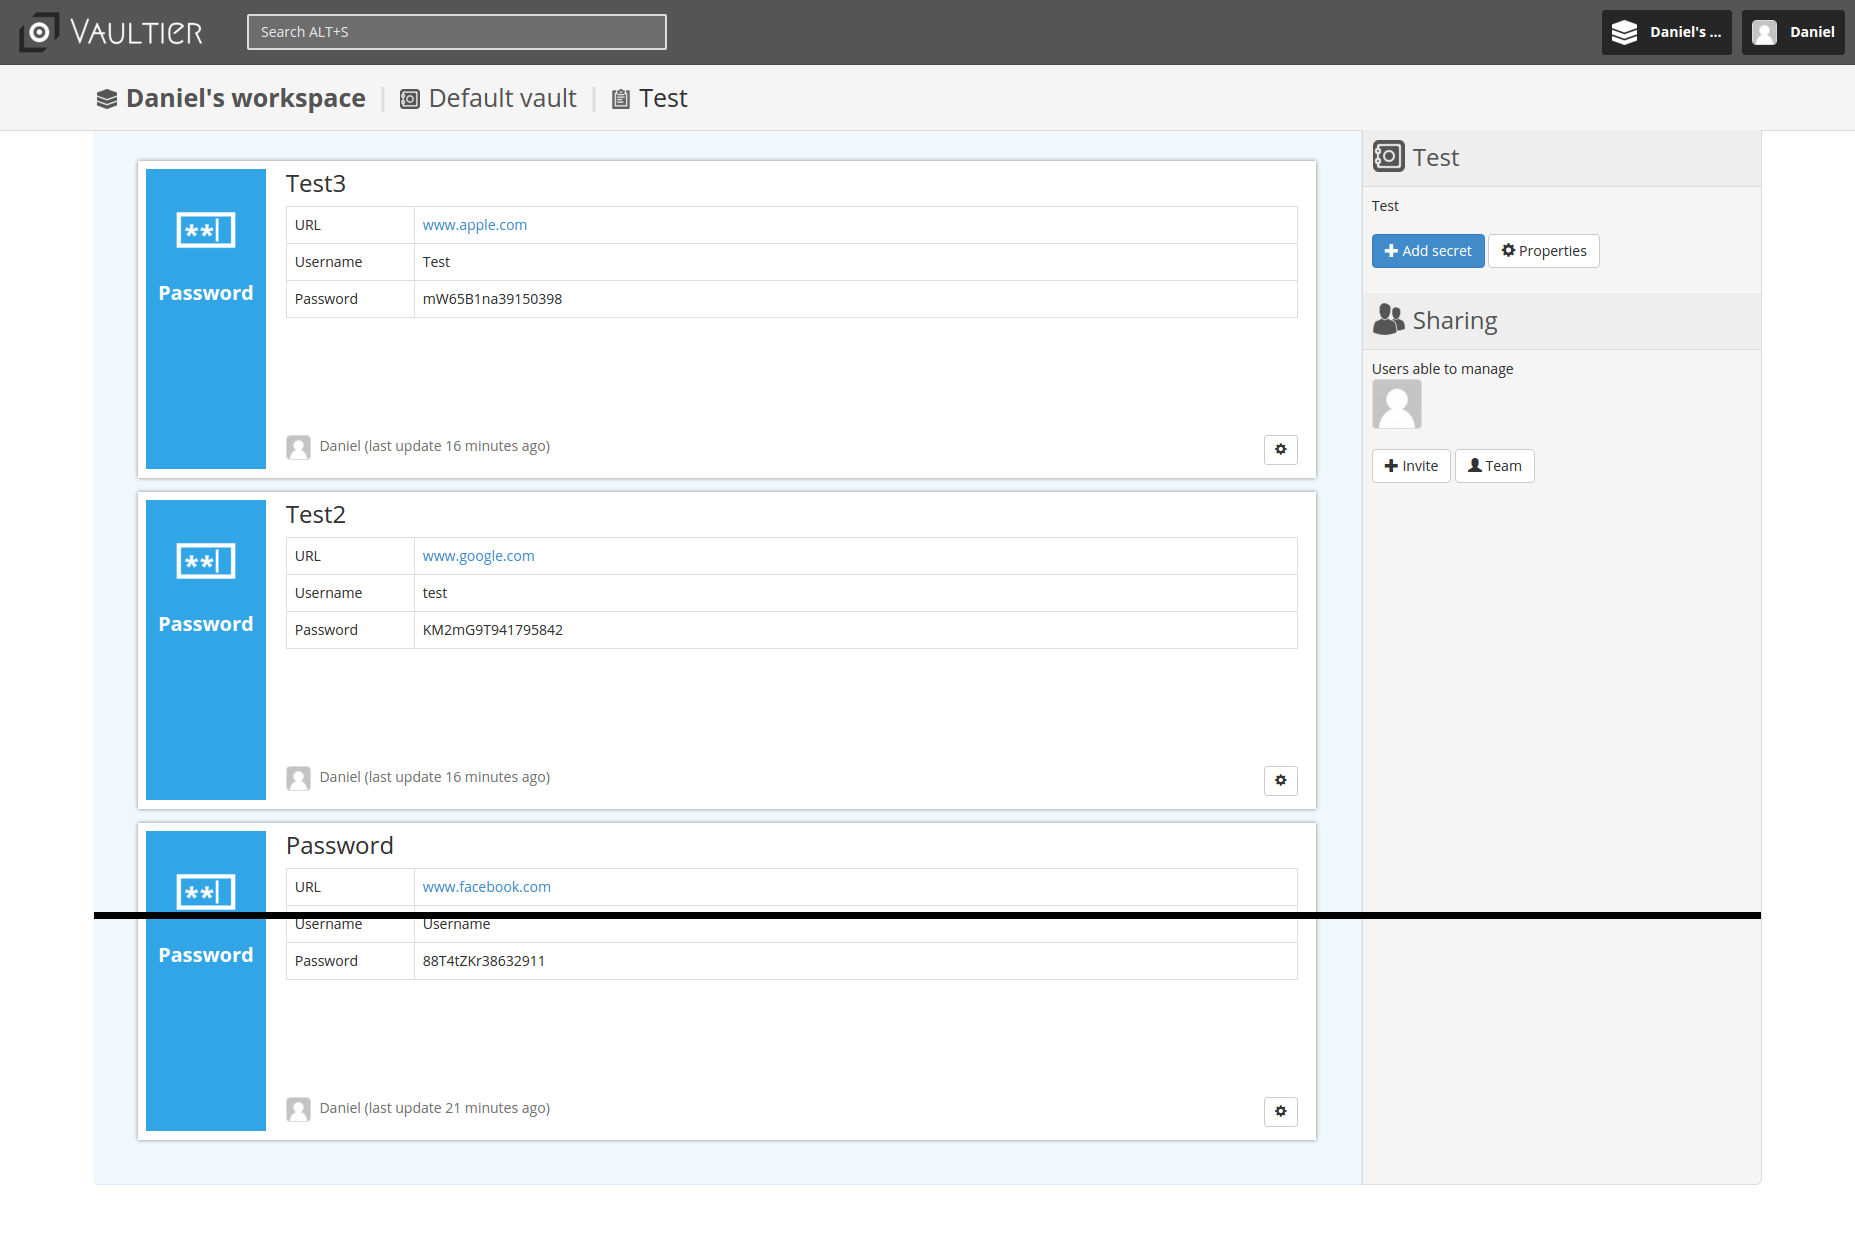
\includegraphics[width=0.95\textwidth]{figures/analysis/vaultier_passwords_lined.png}
				\caption{List of available passwords inside a card, in Vaultier. The dotted line represents the bottom of the browser window, maximized on a 1080p screen.}
				\label{fig:vaultier_passwords}
			\end{figure}
			\begin{figure}[htbp]
				\centering
				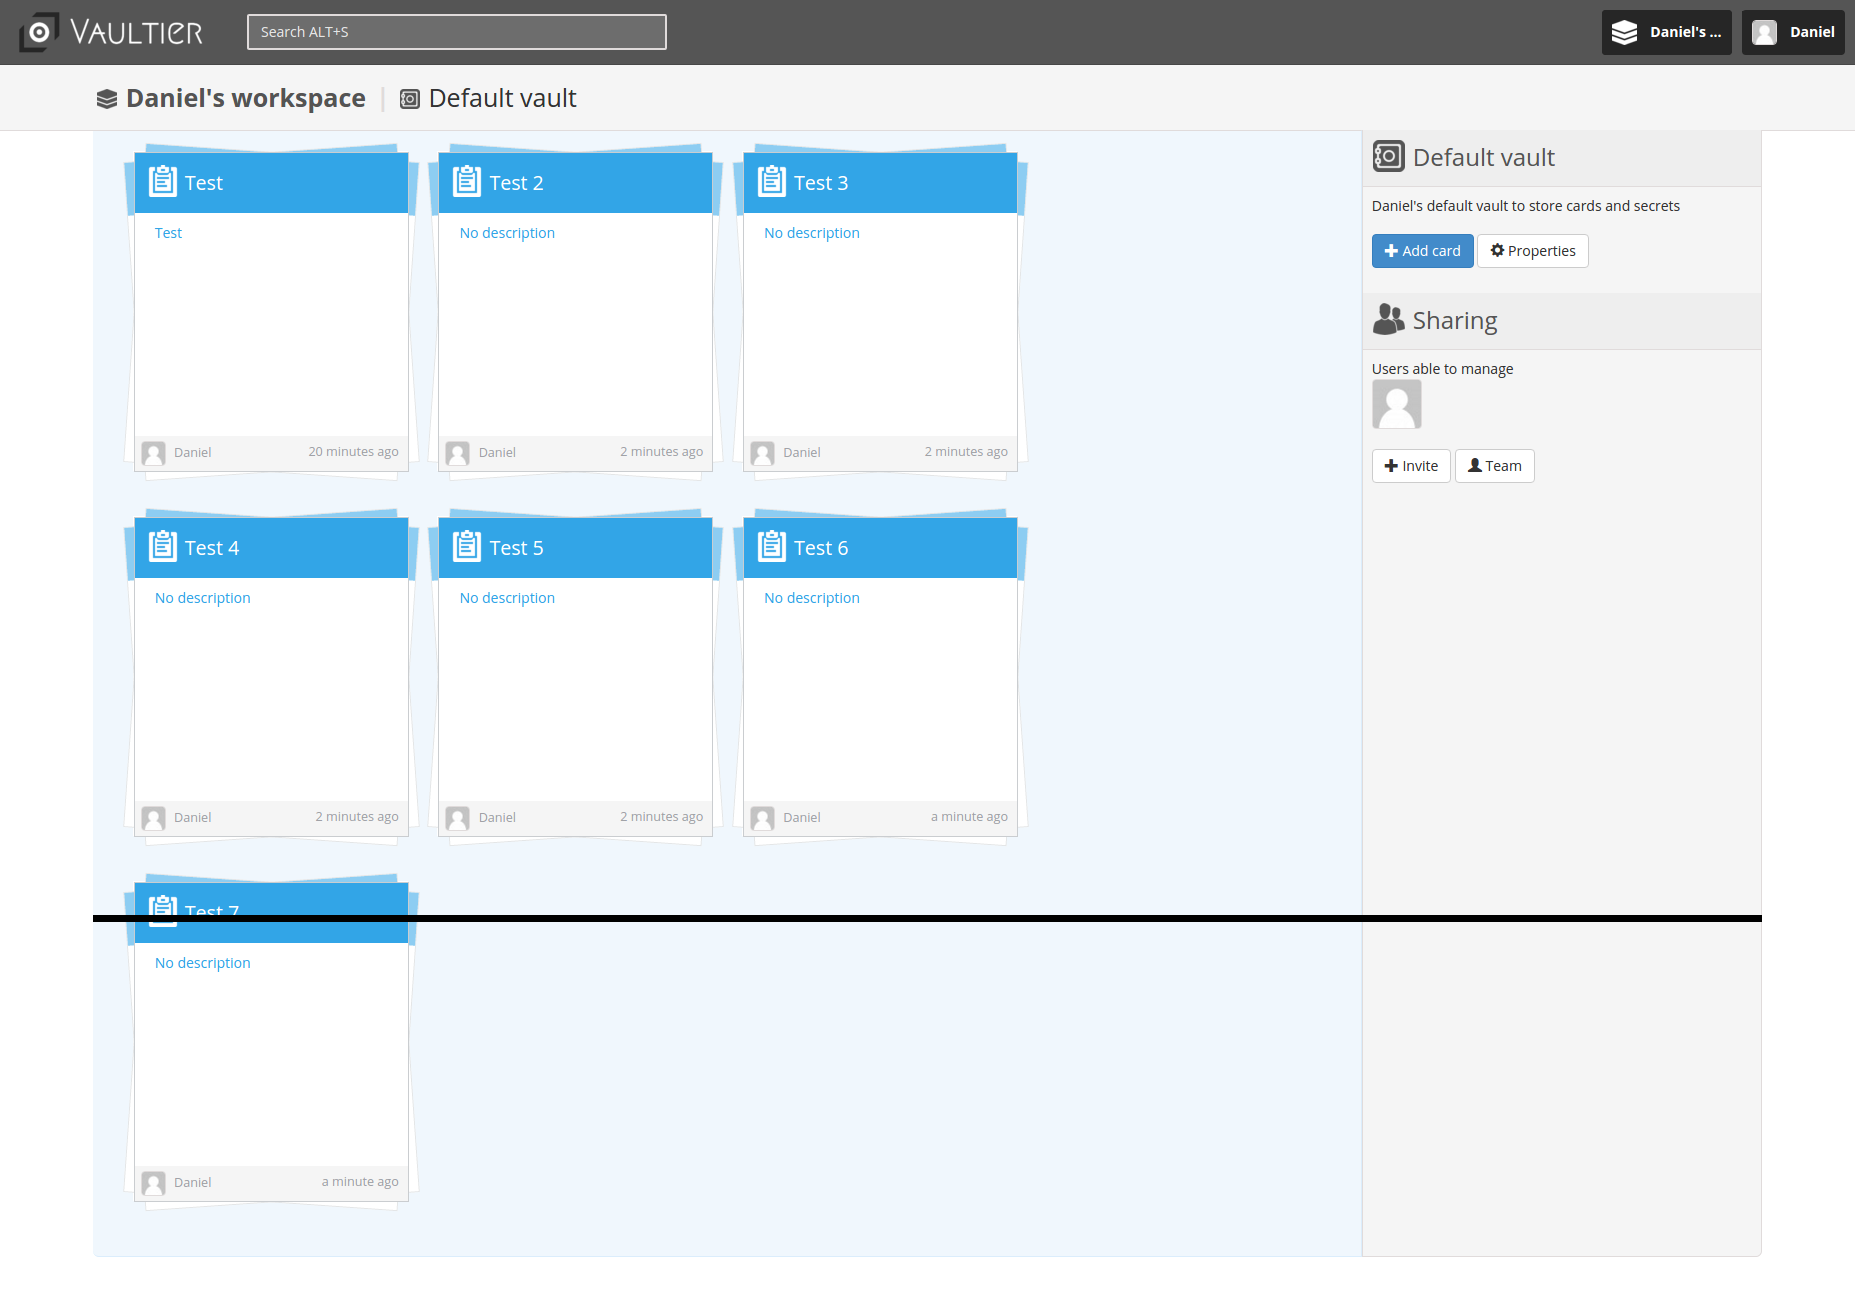
\includegraphics[width=0.95\textwidth]{figures/analysis/vaultier_cards_lined.png}
				\caption{List of available cards inside a vault, in Vaultier. The dotted line represents the bottom of the browser window, maximized on a 1080p screen.}
				\label{fig:vaultier_cards}
			\end{figure}

		\subsection{Final Comparisons}
			% Table color shortcuts
			\newcommand{\red}[1]{\cellcolor{red!75}#1}
			\newcommand{\green}[1]{\cellcolor{green!75}#1}
			\newcommand{\grey}[1]{\cellcolor{gray!75}#1}
			\newcommand{\yellow}[1]{\cellcolor{yellow!75}#1}


			While the previous sections covered an in-depth look at the various solutions, it might seem a little overwhelming. Here, the information will be condensed into tables, for a better picture of the differences between the various solutions.

			First and foremost, on table \ref{tbl:web_based} on page \pageref{tbl:web_based}, a clear cut distinction is seen: The solutions that are \emph{able} to be run in the private cloud, and those who isn't. Focussing only on those which actually \emph{can} exist in the private cloud, on table \ref{tbl:passwords} on page \pageref{tbl:passwords} their default approach to passwords are compared. While all of the systems support multiple users in \emph{some} way, they all pretty much share the same sigh on personal passwords: They should not exist. This is primarily a result of nearly all of these being marketed towards teams. For almost all of the solutions, the same approach to solving this shortcoming is the same: Create a new \emph{personal} group for each individual user, in which personal passwords can be stored. Unfortunately, this \emph{must} be considered a workaround, with the exception of PassWork, in which this group is created automatically. 

			Looking at the more technical aspect of the comparison, on table \ref{tbl:agnostic} on page \pageref{tbl:agnostic} a comparison of their agnosticism is made. Most of the solutions are able to be run on multiple platforms, due to being implemented in PHP. Hence, they only require an Apache \emph{(or nginx)} server to be run. Fortunately, both of these have versions for all major operating systems. Unfortunately, there is only one solution that actually has options for various database solutions. \emph{But} the developers note, that this is done at the user's risk, since they're not tested as rigorously.

			By comparing these three tables, it is unfortunately seen that there isn't \emph{one} completely fulfilling the requirements earlier specified.



			\begin{table}
				\begin{minipage}{1.0\textwidth}
					\begin{tabular}{| r | l | l |}
						\hline
						Name 						& Web Based 			& Self-Hostable 		\\
						\hline
						LastPass 					& \green{Yes}			& \red{No} 				\\
						\hline
						KeePass 					& \red{No} 				& \grey{N/A} 			\\
						\hline
						Rattic 						& \green{Yes} 			& \green{Yes}  			\\
						\hline
						Encryptr 					& \red{No} 				& \yellow{Yes} \footnote{Requires editing source files and running own Crypton backend.} 			\\
						\hline
						Passwordstate 				& \green{Yes} 			& \green{Yes}  			\\
						\hline
						Vault \emph{(Zoho)} 		& \green{Yes} 			& \red{No} 				\\
						\hline
						TeamPasswordManager 		& \green{Yes} 			& \green{Yes}  			\\
						\hline
						Simple Safe 				& \green{Yes} 			& \green{Yes}  			\\
						\hline
						Passwork 					& \green{Yes} 			& \green{Yes}  			\\
						\hline
						SimpleVault 				& \green{Yes} 			& \green{Yes}  			\\
						\hline
						RoboForm 					& \red{No} 				& \grey{N/A} 			\\
						\hline
						TeamPass 					& \green{Yes} 			& \green{Yes}  			\\
						\hline
						Vaultier 					& \green{Yes} 			& \green{Yes}  			\\
						\hline
					\end{tabular}
				\end{minipage}
				\caption{Comparison of access method and ownership model, of the available solutions.}
				\label{tbl:web_based}
			\end{table}


			%% Footnotes for Table tbl:agnostic
			\newarray\tblPasswordsFN
			\tblPasswordsFN(1)={Through password grouping.\label{fn:passwords:group}}
			\tblPasswordsFN(2)={Through a commonly used master passphrase, acting as a work-around.\label{fn:passwords:common_masterpassphrase}}
			\tblPasswordsFN(3)={By each user, using their own unique passphrase for encrypting their personal passwords.\label{fn:passwords:unique_masterpassphrase}}
			\begin{table}
				\begin{minipage}{1.0\linewidth}
					\begin{tabular}{ | p{0.30\textwidth} | p{0.25\textwidth} | p{0.15\textwidth} | p{0.15\textwidth} | }
						\hline
						\textbf{Name}  		& \textbf{Supports Multiple Users} 			& \textbf{Personal Passwords} 					& \textbf{Password Sharing} \\
						\hline
						Rattic 				& \green{Yes} 								& \yellow{Yes}\footnote{\tblPasswordsFN(1)}		& \green{Yes} 				\\
						\hline
						Passwordstate 		& \green{Yes} 								& \yellow{Yes}\footref{fn:passwords:group}		& \green{Yes}				\\
						\hline
						TeamPasswordManager & \green{Yes} 								& \yellow{Yes}\footref{fn:passwords:group}		& \green{Yes}				\\
						\hline
						Simple Safe 		& \green{Yes} 								& \yellow{Yes}\footref{fn:passwords:group}		& \green{Yes}				\\
						\hline
						Passwork 			& \green{Yes} 								& \green{Yes}									& \green{Yes}				\\
						\hline
						SimpleVault 		& \yellow{Yes}\footnote{\tblPasswordsFN(3)} & \green{Yes}\footref{fn:passwords:unique_masterpassphrase}		& \yellow{Yes}\footnote{\tblPasswordsFN(2)}\\
						\hline
						TeamPass 			& \green{Yes} 								& \yellow{Yes}\footref{fn:passwords:group}		& \green{Yes}				\\
						\hline 				
						Vaultier 			& \green{Yes} 								& \yellow{Yes}\footref{fn:passwords:group}		& \green{Yes}				\\
						\hline
	   				\end{tabular}
	   			\end{minipage}

				\caption{Comparison of password ownership in self-hostable solutions.}
				\label{tbl:passwords}
			\end{table}



			%% Footnotes for Table tbl:agnostic
			\newarray\tblAgnosticFN
			\tblAgnosticFN(1)={Databases other than MySQL receives less testing.}
			\tblAgnosticFN(2)={No information available to determine.\label{fn:agnostic:no_info}}
			\tblAgnosticFN(3)={Doesn't use a database. Stores passwords in a .txt file.}

			\begin{table}
				\begin{minipage}{1.0\linewidth}
					\begin{tabular}{|r | l | l|}
						\hline
						Name 				& Platform Agnostic 						& Database Agnostic 						\\
						\hline
						Rattic 				& \green{Yes} 								& \yellow{Yes}\footnote{\tblAgnosticFN(1) } \\
						\hline
						Passwordstate 		& \red{No} 									& \red{No} 									\\
						\hline
						TeamPasswordManager & \green{Yes} 								& \red{No} 									\\
						\hline
						Simple Safe 		& \green{Yes}  								& \red{No} 									\\
						\hline
						Passwork 			& \grey{N/A}\footnote{\tblAgnosticFN(2)} 	& \grey{N/A}\footref{fn:agnostic:no_info} 	\\
						\hline
						SimpleVault 		& \green{Yes} 								& \red{No}\footnote{\tblAgnosticFN(3)} 		\\
						\hline
						TeamPass 			& \green{Yes} 								& \red{No} 									\\
						\hline
						Vaultier 			& \green{Yes} 								& \red{No} 									\\
						\hline
					\end{tabular}
				\end{minipage}

				\caption{Comparison agnosticism of self-hostable solutions.}
				\label{tbl:agnostic}
			\end{table}
	
	\section{Academic Research and Tools}
		A number of interesting academic articles and papers was discovered, while researching available solutions from this source. The findings of this, has been condensed into the following list.

		\begin{itemize}
			\item Tapas: Design, Implementation, and Usability Evaluation of a Password Manager \cite{tapas}
			\item Using CardSpace as a Password Manager \& Implementing PassCard - a CardSpace-based Password Manager \cite{cardspace,cardspace_impl}
			\item Stronger Password Authentication Using Browser Extensions
			\item Kamouflage: Loss-Resistant Password
			\item Sesame: A Secure and Convenient Mobile Solution for Passwords
			\item All Your Browser-saved Passwords Could Belong to Us: A Security Analysis and a Cloud-based New Design
			\item Cloud Based Manager Using Privacy-Preserved Biometrics
		\end{itemize}
		

		\subsection*{Tapas: Design, Implementation, and Usability Evaluation of a Password Manager}
			In \cite{tapas}, a new and novel idea is introduced. Rather than using two-factor authentication, a \emph{dual-possession} authentication is used. The basic concept is, that the user has two devices: A smartphone \emph{(wallet)} and a desktop \emph{(manager)}. While it \emph{specifically} states that the manager is a desktop, it is assumed that it might as well be a laptop. The idea is that the manager stores keys for decrypting login information to various sites, while the wallet stores encrypted blobs. The argument is, that even if either device is stolen, offline attacks cannot happen.

			The authentication for storing and retrieving passwords is then based on the fact that the user is in possession of \emph{both} devices, at the time of login. As they describe their solution, it is only possible to access and use passwords on the manager, while the wallet actually stores them. The proposed protocols are:
			\begin{itemize}
				\item Pairing Manager and Wallet
				\item Storing a Password
				\item Retrieving a Password
			\end{itemize}

			Tapas relies on so-called pairing, for easy authentication between wallet and manager, in the remaining protocols. The pairing has to be done in a secret out-of-band channel. During this pairing a private and public key for each device is created, and the public key for the manager is sent to the wallet, and vice versa. This ensures that a secure channel, over a possible hostile connection, can be made in the future.

			While the protocol for storing a password is hardly interesting, the protocol for retrieving a password does present an interesting approach. Retrieval of a password has to be initiated on the \emph{wallet}, or rather smartphone. After authenticating using the previously obtained public keys, they create a secure channel, with perfect forward secrecy, and the wallet sends the encrypted blob to the manager, which then decrypts it and auto-types it in the users browser.

			The team behind Tapas is fairly open regarding what \emph{they} consider the limitations of Tapas. As they see it, there are tree major. First and foremost, the solution relies on an active internet connecting for retrieving passwords. This limitation is unfortunate, but unavoidable with their choice of authentication. It is, however, easily avoided by use of USB tethering or WiFi hotspots, which are standard features in modern smartphones. Secondly, their other limitation is that the smartphone must be charged. Again, a very unavoidable limitation, due to how technology works. The last, and perhaps the only real concern, other than small inconveniences is the fact that Tapas does \emph{not} support multiple devices. It only works with \emph{one} wallet and  \emph{one} manager. Even the wallet cannot access these passwords which is unfortunate, since a lot of the same accounts for a desktop, is also used on a smartphone. All in all, renders it as an unsuited approach to the problem at hand.

		\subsection*{Using CardSpace as a Password Manager \& Implementing PassCard - a CardSpace-based Password Manager}
			In \cite{cardspace,cardspace_impl} the authors design and implement PassCard: A password manager based on CardSpace. CardSpace was Microsoft's client software for their ``Identity Metasystem''. The program was retired as of February 15th 2011, but Microsoft stated that they are working on a replacement \cite{cardspace_cancelled}. This is a service that was discontinued in 2011, and has not been shipped with windows since Windows 8.0. This alone, indicates that this solution is not suitable for any modern devices.

			The basic concept of PassCard, is that the user creates ``Personal Cards''. These cards are able to store various sensitive information, securely. Their solution is a browser extension, which then reads these cards and auto-fills the information. No where in their report, do they describe anything related to adding passwords through PassCard, which leads to believe that his has to be done manually, directly in CardSpace.

			Since CardSpace is a windows only program, this limits the user segment significantly. Additionally, the paper does not mention whether or not they support any kind of multi-device operation, but even if it did it would more than likely be limited to Windows platforms. Hence, the solution is \emph{unusable} for mobile devices, and users of either Mac OS X or Linux. All in all, this solution seems poor in comparison to what we've seen.

		\subsection*{Stronger Password Authentication Using Browser Extensions}
			In \cite{pwdhash} the implementation of PwdHash is discussed. PwdHash's approach, is using a browser plugin as password manager. Their primary issue, seems to be the issue of sending a cleartext password to a remote server for sign up. Their proposal is centered around password derivation, rather than password generation. When typing the password to a site, PwdHash intercepts the password and creates a derived password, using an un-named pseudo random function. The new password is derived from the users original password and the domain name of the site. This derived function is then input into the password field on the website, and the user has retrieved a secure password seamlessly. Salting with the domain name, ensures that even if the user uses the same password for all websites, a unique password is submitted to each site.

			In the paper, the authors make a point of describing each of their steps for avoiding various attacks. Their solution relies on a ``traffic light'', as they call it. When this is green, the user is inputting a password. When it is red, the user is inputting other -- insecure -- information. 

			Additionally, they suggest that the user either inputs a password-prefix, or uses a ``password-key''. Their example of a prefix is \verb=@@=, which the user would have to type every time he or she logged into a site. As an alternative, they suggest using a dedicated keyboard, which they call a ``password-key'', with a button called \verb=password=. In their prototypes they use the \verb=F2= key as a password key.

			To support devices that does not support plugin development, they have a website set up to derive a password, based on a user password and the URL of the website. Additionally they suggest developing a bookmarklet, down the road. As previously discussed, bookmarklets are essentially a security hazard disguised as a usability feature, and should be avoided for all costs.


			After reviewing the paper thoroughly, it is concluded that PwdHash is much more of a secure password derivation tool, rather than an actual password manager. The horrible fact is, that the user still has to input a password for each login. Since users are -- at heart -- lazy, it can be assumed with a fair degree of accuracy, that the majority will re-use the same password over and over. Hence, the only security is that the password is hashed with a \emph{predictable} and very public hash \emph{(the domain name)}. If an attacker was to discover the base password for one site, he or she would then potentially get access to all the users passwords \emph{(assuming the user is lazy)}.

			If, somehow, the user was \emph{not} lazy and had unique passwords for each site, the original problem would still persist. There would be so many unique passwords to remember, that they would be extremely easy to crack using wordlists or simple bruteforce.

			Finally, despite all of their analysis regarding attacks on remote sites, they fail to see that \emph{all} of the same attacks applies to their website for deriving passwords, rendering it a security hazard.

			All in all, PwdHash is not a solution suited for the problem at hand, and actually does nothing for the usability of secure passwords.

		\subsection*{Kamouflage: Loss-Resistant Password}
			In \cite{kamouflage} a whole new paradigm for creating encrypted password databases is suggested: Kamouflage. Kamouflage relies on what they call decoy password sets. One of their primary arguments for implementing Kamouflage is the fact that you can't trust the cloud. Their concern is, that an employee at the cloud service could download the DB and run offline attacks against it. However, they neglect to reason against running this cloud service yourself.

			Imagine a user having a set of passwords, $S$. Then, Kamouflage generates $N$ additional sets, $S_1, \dots S_{N-1}$ to work as decoy password sets. They suggest a default value of $N=1000$. These passwords are generated, using an algorithm based on the work in \cite{cracking}. The aim is generate passwords which are statistically indistinguishable from the \emph{actual} passwords. 

			All of these sets, are then stored side-by-side, in a single file. The idea is then, that the users master password can be run through a cryptographic function and return and index into the file. This index, is then where the \emph{real} password set is stored. A wrong master password would result in another index, which again would result in a decoy password.

			They argue, that with the help of online services, these decoy password sets could be able to be used to detect targeted attacks. However, this both requires that the major websites actually chooses to adopt this technology themselves, and that they need to maintain at least \emph{some} of these passwords on their servers, increasing the needed storage by a decent factor.

			Their scheme for applying encryption to this structure is somewhat convoluted. For each set, they create a password relating to the contents. The algorithm for generating this password, is the same as earlier mentioned. Then, using this password, an encryption key is generated. This key is then used to encrypt the set. After successful encryption of a decoy set, the key is deleted. For the \emph{real} set, the users master password is used to generate an encryption key.

			As the paper states, the layout of the encrypted file, is supposed to make it more difficult for an attacker to access the \emph{correct} password, using offline attacks. Based on this, it appears as if the idea behind Kamouflage is that the encrypted file is stored locally. While their idea of decoy sets might be novel and could potentially be a boost in security, their solution does \emph{nothing} towards solving the problem at hand.

		\subsection*{Sesame: A Secure and Convenient Mobile Solution for Passwords}
			In \cite{sesame} a rather novel idea regarding password managers is described. While the core of Sesame differs in no way from the different solutions described, the process of unlocking the database is where it differs.

			Sesame can be unlocked using voice recognition. Using a remote server, a piece of recorded voice can be used to unlock the password manager. While on a desktop this might be considered unnecessary, it does save the user some hassle of typing in a password on mobile devices.face

			While the idea is novel, and some user might find it exciting and usable, it is fairly limited in regards to platforms. As the authors write themselves, it is intended for smartphones, tablets, smartwatches etc. Hence, the usage for the problem at hand is rather limited.

		\subsection*{All Your Browser-saved Passwords Could Belong to Us: A Security Analysis and a Cloud-based New Design}
			In \cite{browser_saved} they suggest a solution to fix the issues the found, as mentioned in section \ref{subsec:in-browser}. They argue that the data is more secure on a remote machine, run by a company. They prefer to rely on a ``Secure \& Reliable Storage'' service, located in the cloud. They have developed an encryption scheme aimed at protecting the passwords of the users, even though they are stored on a remote machine. 

			However, no matter how secure their scheme is, their suggestion goes against some of the very fundamental requirements mentioned in section \ref{sec:requirements}. As such, their solution is dismissed as not suitable for this specific purpose. 

		\subsection*{Passpet: Convenient Password Management and Phishing Protection}
			In \cite{passpet} a system for managing passwords is suggested: Passpet. It revolves around the idea of petnames. The first time the user uses Passpet, he or she is given a ``persona''. This persona, is essentially a pet, consisting of a random animal logo \emph{(selected from a set of logos)} and a random name. An example of this, is Betty the Fish, as seen on figure \ref{fig:passepet_persona} on page \pageref{fig:passepet_persona}. The randomness is introduced in an attempt to avoid phishing attacks, as the attacker can never know exactly which logo and what name, has been assigned to the user.

			They describe a weird combination of both deriving a password, based on site information and storing data remotely. They derive a password based on a master address \emph{(address of a remote Passpet server)}, a master secret, two constants $k_1$ and $k_2$, and a site label.

			Using passpet only requires the user to press a button, once the correct site label has been entered. This is seen on figure \ref{fig:passpet_main} on page \pageref{fig:passpet_main}.


			\begin{figure}[htbp]
				\centering
				\includegraphics[width=0.95\textwidth]{figures/analysis/passpet_persona.png}
				\caption{Creation of a Passpet persona. \textbf{Source:} \cite[p.4]{passpet}.}
				\label{fig:passepet_persona}
			\end{figure}

			\begin{figure}[htbp]
				\centering
				\includegraphics[width=0.95\textwidth]{figures/analysis/passpet.png}
				\caption{Using Passpet. \textbf{Source:} \cite[p.1]{passpet}}
				\label{fig:passpet_main}
			\end{figure}

			Unfortunately, there is an ambiguity in the paper. Several places, a ``Passpet server'' is mentioned, however it is never specifically told who owns this server. 

			To access passwords on other devices, the user will have to input the master address and master secret, and the remote machine will store the constants along with the label list, in order to recreate the passwords. Their description of how a user is authenticated for a second device is poorly described.

			This solution suffers from the same basic issue as described in section \ref{subsec:in-browser}: It only works for website logins, and only in the browser the plugin supports. This, combined with the ambiguity of their report leads to the conclusion that their solution is unfit to solve the problem at hand.


		\subsection*{Cloud Based Manager Using Privacy-Preserved Biometrics}
			Most solutions examined so far, has had the same approach to storing these password databases: Protect them behind a master password. In \cite{busch2014}, however, they argue for another approach: Use biometrics for authenticating access. Building on the prior work of Jain, Nandakumar, and Nagar, they employ Biometric Template Protection, to ensure that the original biometric characteristic can not be reverse engineered. This is then used, to authenticate to the cloud, containing the passwords.


			While this idea \emph{novel}, the usability is limited by our current technology. It is simply a fact, that not all of our devices are equipped with sensors able to detect biometric characteristics. Additionally, there have been voiced some concerns about using biometrics for authentication. All in all, the usage of their solution is not suitable for the problem at hand.

		\subsection*{A Password Manager that Doesn’t Remember Passwords}
			In \cite{stobert2014} another take a password manager is described. In it, they design and implement a prototype of the software Versipass. Much like the previous section, Veripass has a novel take on authenticating the user, in order to access the password database.

			Existing as a bookmarklet, Veripass presents the user with an image cue, to verify the user. In short, an image cue is a image based password. An image is divided up into a $6x8$ squares \emph{(default settings)}. A password is then a selection of these squares. An example of this, is seen on figure \ref{fig:versipass_imagecue} on page \pageref{fig:versipass_imagecue}. The squares are chosen at random, by the system. The use of randomly assigned squares, is done to avoid what they call hotspots in the images, which essentially is areas of a picture which is more likely to be chosen by users, than other areas. 

			In order to go from a set of squares into a text-based password, each tile is assigned a a string. These strings are then concatenated into a single string, in a fixed order. The resulting string is then salted and hashed, which then returns the password. In contrast to popular approach, the salt in this process is \emph{ partially user selected}. The salt consists of a combination of the sites URL and a user selected salt. This is done in order for the user to be able to change the password for a site, should it be required.

			From a security perspective, there are some shady aspects of their paper. In section 5.1.1 they cite that 21 bits of ``entropy'' is sufficient for an online attack,and quotes \cite{florencio2014}. However, there is a much more frightening problem: Combinations. In their default settings they state that a $5x6$ grid in which 5 tiles are to be selected, in any order, is sufficient. However, ignoring the advanced analysis

			Applying some math, it is evident that there exists $1712304$ different combinations using these settings, cf. equation \ref{eq:combinations}. At first glance this might seem decent, but in fact it offers \emph{less} combinations than a randomly selected $6$ character long password, consisting \emph{only} of lower-case letters, cf. equation \ref{eq:permutations}. While they do say, that the settings suggested them can be altered to increase security, it still feels like a less secure approach.

			\begin{equation}
				c = \frac{n!}{(n-r)!(r!)} = \frac{48!}{(48-5)!(5!)} = 1712304
				\label{eq:combinations}
			\end{equation}

			\begin{equation}
				p = n^r = 11881376
				\label{eq:permutations}
			\end{equation}

			\begin{figure}[htbp]
				\centering
				\includegraphics[width=0.95\textwidth]{figures/analysis/versipass_imagecue.png}
				\caption{Versipass' image cue password. \textbf{Source:} \cite[p.3]{stobert2014}.}
				\label{fig:versipass_imagecue}
			\end{figure}

			Abstracting away from some of the details, this solution is sort of a parallel to the one described in \cite{busch2014}. While the mechanism for unlocking the password is novel, it is just impractical. Hence, it is deemed as an unsuitable solution for the problem at hand.

		\subsection*{Password Management Using Doodles}
			Much in line with the previously described solutions, \cite{doodles} describes a novel take on the password manager. Their idea is to use doodles to log into websites.

			The basic concept is the same as has been seen over and over again; Username, passwords, and site URLs are stored in a database. Accessing these usernames and passwords, requires the user to draw his or her master doodle in a supplied browser plugin, seen on figure \ref{fig:doodle}. If this entered doodle then is a match with a stored ``master doodle'', the username and password is autofilled.

			Unfortunately, they do not disclose how exactly the database is protected. Additionally, the paper makes no effort taking multiple devices into account. As such, their solution is dismissed.

			\begin{figure}[htbp]
				\centering
				\includegraphics[width=0.95\textwidth]{figures/analysis/doodle.png}
				\caption{The Doodle browser plugin}
				\label{fig:doodle}
			\end{figure}

		\subsection*{Other Sources}
			In \cite{halderman2005} they discuss deriving site specific passwords, from a single master password and a site URL. This is done by hashing the concatenated strings, and the resulting hash is then the password for that specific site. This is a solution very similar to the one described in \cite{pwdhash}.

			In \cite{zhang2015} they have some of the same thoughts, as in \cite{pwdhash}, using a dedicated key to signal TrustLogin that confidential information is being entered. However, it differs from PwdHash as TrustLogin does not actually \emph{store} anything. It is ``merely'' a tool for secure input, on a possibly insecure platform. While their paper doesn't describe a password manager as seen previously, it does presents some interesting takes on securing the input of the user.

			In \cite{englert2009} they describe a very classical password management system: An HTTP server and a browser client. The client logs into the server, gets the encrypted data, and decrypts it locally. However, from their description of the system, the encryption key -- or as they call it the ``secret key'' -- is something the user is supposed to remember and input \emph{per} session. 

			\cite{huang2015} describes what they call a Searchable Conditional Proxy Re-Encryption scheme. Their solution, CloudKeyBank, is based on this SC-PRE scheme is claimed to not only guarantee confidentiality and privacy of the users keys, but also ensuring the privacy in regards to other attributes to each key, amongst others. However, part of their assumptions is the use of a CloudKeyBank provider, i.e. a third party, much like services such as LastPass. As such, their solution is primarily focussed on ensuring that no other person than the owner, can access data even when uploaded to third party servers.
\chapter{Designing the System}
	In the following chapter, the overall design of the system is discussed. First and foremost, the basic architechture is decided, based on the requirements. Then more detailed subjects are covered, such as how authentication will work, how the solution keeps the users' data safe, and generally how it will work under the hood - so to speak.

	\section{Architecture}
		As per the requirements specified in section \ref{sec:requirements} on page \pageref{sec:requirements} the solution will have to be distributed. As such, there are two primary basic paradigms which can be used: Peer-to-Peer and Client-Server. In the following sections the pros and cons of the two will be discussed, and a conclusion of which is more beneficial for the project will be made.

		\begin{figure}
			\centering
			\includegraphics[width=\textwidth]{figures/design/PeerToPeer.pdf}
			\caption{Peer-to-Peer structure visualised.}
			\label{fig:peertopeer}
		\end{figure}

		\begin{figure}
			\centering
			\includegraphics[width=\textwidth]{figures/design/ClientServer.pdf}
			\caption{Client-Server structure visualised.}
			\label{fig:clientserver}
		\end{figure}


		\subsection{Peer-to-Peer}
			Over the past few years, peer-to-peer technology has become ever so more appealing to the masses. Applications such as BittorrentSync applies peer-to-peer technology in an effort to synchronise data between devices. Such an approach could easily be adapted to the problem at hand. A number of a user's devices are online, and synchronises a local password database file between themselves, as visualised on figure \ref{fig:peertopeer} on page \pageref{fig:peertopeer}. This file is then accessed through a native application, on the target device. 

			This approach \emph{definitely} has the lowest overhead of the two: After all it is only devices that needs to have access to the passwords, that need to be setup, maintained, and running for it to be used. However, it does have some drawbacks. Most noticeable, that a native application is required for it to work. This means that for \emph{all} platforms an application needs to be developed. This, in returns, results in a much larger codebase, higher risk of bugs, and a risk of lower consistency across devices. Furthermore, the requirements of logging, as per section \ref{sec:requirements} on page \pageref{sec:requirements}, becomes a lot more difficult, if not to say impossible.

			Additionally, there is a pitfall using this approach. The synchronization requires at least \emph{one} peer with the newest version, to be online for it to work. Let us imagine a user, Paul. Paul has three devices he wish to synchronize passwords to: A desktop, a laptop, and a smartphone -- a very common scenario! Before leaving for a holiday, Paul updates a password on his desktop, while his laptop is closed. Since the smartphone is online at the time, the password is stored there and Paul is perfectly able to access it on his way to the airport. Since it's a long trip, Paul's smartphone runs out of battery along the way. ``No problem!'', Paul thinks and pulls out his laptop -- but oh no! Since the laptop has been offline ever since he left home, it has not received the updated password. And since it is the only online peer -- the desktop at home is turned off and the smartphone has run out of battery -- he can't fetch the newest version. 

			The scenario presented before, can be somewhat mitigated by creating an ``always on peer''. It is a peer in the network, which is always connected and thus always has the newest version available for other peers. However, doing this very much negates one of the strongest arguments \emph{for} this approach: The lower overhead.

		\subsection{Client-Server}
			The client-server paradigm has been the basic model used, since the dawn of the modern internet. When browsing facebook, accessing gmail, or posting a tweet, this is the paradigm employed. It is also the most widespread model used, by the solutions examined in chapter \ref{chap:analysis}.

			Using this approach, there would have to be a dedicated server, acting as the ``master storage'' of passwords. Each client then connects to this server and fetches the passwords. This type of connection is visualised on figure \ref{fig:clientserver} on page \pageref{fig:clientserver}. This does, however, come with its own drawbacks. Since all passwords are stored on a single server, it introduces the risk of a single point of failure. Should the server be compromised or is otherwise unavailable, passwords can not be retrieved \emph{(unless a local cache is used, but this is delving into implementation details)}. It also comes with overhead in form of cost and maintenance. A server will have to be maintained and run 24/7. However, as mentioned in section \ref{sec:privatecloud_cost} on page \pageref{sec:privatecloud_cost}, this can be achieved using low-power devices such as a Raspberry Pi, reducing the financial cost significantly.

			Finally, using the client-server paradigm counters the scenario presented in the previous section. When Paul updates the password from home, the updated password is stored on the server. When he uses his laptop, after his phone has died, it will fetch the updated password from the server.


		\subsection{Conclusion}
			After having weighed the pros and cons of the two approaches, it is decided that a classic client-server architecture will be used. It is deemed that it will create a more seamless experience for the user, and over all will be a more robust solution.

			Another argument why the client-server paradigm is preferable is that if the peer-to-peer paradigm is used, a native application is \emph{required}. This is not the case for the client-server paradigm. A web UI could serve as a front-end, creating a completely identical user experience across devices. But a native application could also be the solution, for the client-server application. Hence, this paradigm allows more freedom of implementation, than peer-to-peer does.

			From here on out, the solution will be split into two parts: The front-end \emph{(client)} and back-end \emph{(server)} -- two very common denominators.

	\section{Communicating}
		Having determined that the solution will be using the client-server paradigm, the next task is to determine how front-end and the back-end will communicate. There are a number of different available technologies and protocols readily available for use in such a scenario.

		One important fact, that needs to be stated that the back-end is practically equivalent to a web service. As such, 

		\begin{itemize}
			\item Representational State Transfer
			\item SOAP	
			\item Sockets
			\item Remote Procedure Calls
		\end{itemize}

		\subsection{Remote Procedure Call}
			Remote Procedure Calls, or RPC for short, was introduced by Birrell and Nelson \cite{birell1984} in 1984. The basic concept is to hide the implementation details of invoking a method remotely, for the user.

			The core concept of RPC is that invoking remote methods, are no different than invoking a local method. When the program invokes this method, the underlying software then makes the remote call, hiding these details from the programmer. This is the supposed strength of RPC: It is exactly like invoking a local method.

			An example of an RPC method, could be a method to get a user's data:
			\begin{verbatim}
				getUser(<ID>)
			\end{verbatim}

			For simplicity purposes, Remote Method Invocation is considered equivalent to RPC. Likewise implementations of RPC such as XML-RPC, Corba, and so forth, are considered under the same umbrella.

		\subsection{Representational State Transfer}
			Representational State Transfer, or REST for short, was introduced by Fielding and Taylor \cite{Fielding:2000:PDM:337180.337228} in 2000. REST is an architecture style for designing networked application. It is a stateless, client-server communication \emph{style}, which in most cases uses the Hypertext Transfer Protocol \emph{(HTTP)} protocol and the accompanying HTTP ``verbs''. Traditionally REST uses JSON as body encoding, however it is also possible to use XML.

			The core notion of REST is that resources are bundled in collections, on which the HTTP verbs are used. The API then exposes these collections as Uniform Resource Identifiers \emph{(URIs)} in what is commonly known as endpoints. Using the various HTTP verbs on these endpoints results in actions being invoked on said collections.

			These verbs are for example -- but not limited to-- \verb=GET=, \verb=POST=, \verb=PUT=, \verb=PATCH=, and \verb=DELETE=. These five verbs roughly translates to the basic CRUD operations, as listed on table \ref{tbl:verbs} on page \pageref{tbl:verbs}. So, for instance if one where to \verb=GET= the endpoint of \verb=/api/users= one would get the list of all users on the system. However, most of the time the distinction between \verb=PUT= and \verb=PATCH= is ignored, and \verb=PUT= is allowed to perform partial updates. Table \ref{tbl:rest_example} on page \pageref{tbl:rest_example} shows an example of an API on the \verb=users= resource, showing the result of the respective verbs and their payload. In the example the host of the endpoints have been removed, the prefix could for example be \verb=https://someapi.com/api=, so that an endpoint would be \verb=https://someapi.com/api/users=.

			\begin{table}
				\begin{tabular}{r|l}
					\verb=GET= 		& Read 				\\
					\verb=POST= 	& Create 			\\
					\verb=PUT= 		& Complete update 	\\
					\verb=PATCH= 	& Partial update 	\\
					\verb=DELETE= 	& Delete 			\\
				\end{tabular}

				\caption{How HTTP verbs maps to CRUD operations.}
				\label{tbl:verbs}

			\end{table}

			\begin{table}
				\begin{tabular}{p{0.15\textwidth} | p{0.30\textwidth} | p{0.15\textwidth} | p{0.25\textwidth}}
					Method & Request Body & Endpoint & Ouput \\
					\hline
					\verb=GET= & Empty & /api/users & List of all users \\
					\hline
					\verb=GET= & Empty & /api/users/1 & Details of user with ID of 1 \\
					\hline
					\verb=POST= & \{username:"Daniel", phone:"+45 88888888"\} & /api/users & Creates a new User with the name Daniel and the phone number +45 88888888 \\
					\hline
					\verb=PUT= & \{username:"John"\} & /api/users/1 & Updates the username of the user with ID of 1\\
					\hline
					\verb=DELETE= & Empty & /api/users/1 & Deletes the user with ID of 1\\
				\end{tabular}

				\caption{Example of HTTP verbs used on a REST API for the collection of users.}
				\label{tbl:rest_example}

			\end{table}

		\subsection{Simple Object Access Protocol}
			Simple Object Access Protocol \emph{(SOAP)} was developed by Goshein, Atkinson, Winer, and Box for Microsoft in 1997 \cite{soap_origin}. SOAP is considered an extension of XML-RPC and -- like its predecessor -- uses XML encoding. As implied by its successor SOAP is \emph{strictly speaking} considered an RPC, however due to its uniqueness from ``traditional'' RPCs it is considered separately.

			SOAP can be used with any number of protocols, due to its neutrality, however it is usually used with HTTP or SMPT. Web services relying on SOAP, usually publish a public definition of the available methods, using the Web Service Definition Language \emph{(WSDL)}. This can then be consumed by other clients, making integration with third parties much easier.

			Since SOAP used XML encoding, it is \emph{quite} verbose, and the pure data overhead is significant. Using the same example as from REST, getting the information for a user with ID 1 requires a rather large request body. the XML uses multiple namespaces, the \verb=xmlns= tags are required to define each of them, as \verb=SOAP= and \verb=m= respectively.

			\begin{verbatim}
				<SOAP:Envelope xmlns:SOAP="http://schemas.xmlsoap.org/soap/envelope/">
				    <SOAP:Body>
				        <m:getUser xmlns:m="https://someapi.com/api">
				            <userId>41</userId>
				        </m:getUser>
				    </SOAP:Body>
				</SOAP:Envelope>
			\end{verbatim}


		\subsection{Sockets}
			Underlying all of the previously described technologies are sockets. Sockets are the basic method computers communicate with eachother. Hence, of course it can be used for this purpose. However, there is a \emph{reason} the previous technologies exist: They take care of some of the heavy lifting. Defining a standard for communication, redundancy, standard errors, etc. are but some of the advantages of using either of the previously described technologies. As such, using sockets directly is dismissed without further arguments. 


		\subsection{Making A Choice}
			Making the final choice of how the solution will communicate is important. It sets limitation on future work, and could possibly influence design choices not yet even thought of. 

			First and foremost let us examine RPC. While it \emph{was} the go-to method for achieving the sort of communication which is needed in this project, the issue of implementation remains. Each platform will need its own unique implementation of whichever RPC standard that is chosen. And there is no guarantee that all of these will adhere to the specifications. Additionally, since its usage has become less widespread, it will also hinder further development and integration from third parties, down the line. As such, RPC is dismissed as a possible solution.

			This leaves SOAP and REST. SOAP is a very ``heavy'' tool, often used in commercial applications, due to its stricter nature. Because of the XML syntax, their payload is \emph{significantly} larger than that of REST using JSON. This results in SOAP being magnitudes slower than REST, cf. \cite{soap_vs_rest}. Additionally there is the matter of support and general adaptation. In the open-source community REST seems to have won the hearts of the crowd. More libraries and tools exists, for aiding in quick development of a RESTful API. This will also make for the optimal base, should other users choose to integrate the solution with their own projects.

			Hence, it is decided that a RESTful approach will be used.

	\section{Data Protection \& Encryption}
		In this section we will discuss	


		First, it is needed to re-cap two \emph{very} important requirements:
		\begin{enumerate}
			\item Passwords and private information should never be stored or handled un-encrypted anywhere, other than the local device
			\item Password sharing
		\end{enumerate}

		The first requirement states that the passwords needs to be encrypted, when handled in the back-end. Multiple encryption and data schemes could be used for this.

		\subsection{A Single Encrypted Blob}
			One solution, is to simply store \emph{one} large encrypted blob in the back-end. When the user then requests access to a password, this blob is transferred to the front-end, decrypted, and the password can be retrieved. 

			When a new password is generated -- or an old one updated -- the same happens. The front-end fetches the blob, decrypts it, updates or creates an entry, re-encrypts the blob, and then pushes the entire thing to the back-end. The back-end then overrides its own version, with the newly received one. This sequence of events is depicted on figure \ref{fig:seq_blob} on page \pageref{fig:seq_blob}.

			\begin{figure}[h!]
				\centering
				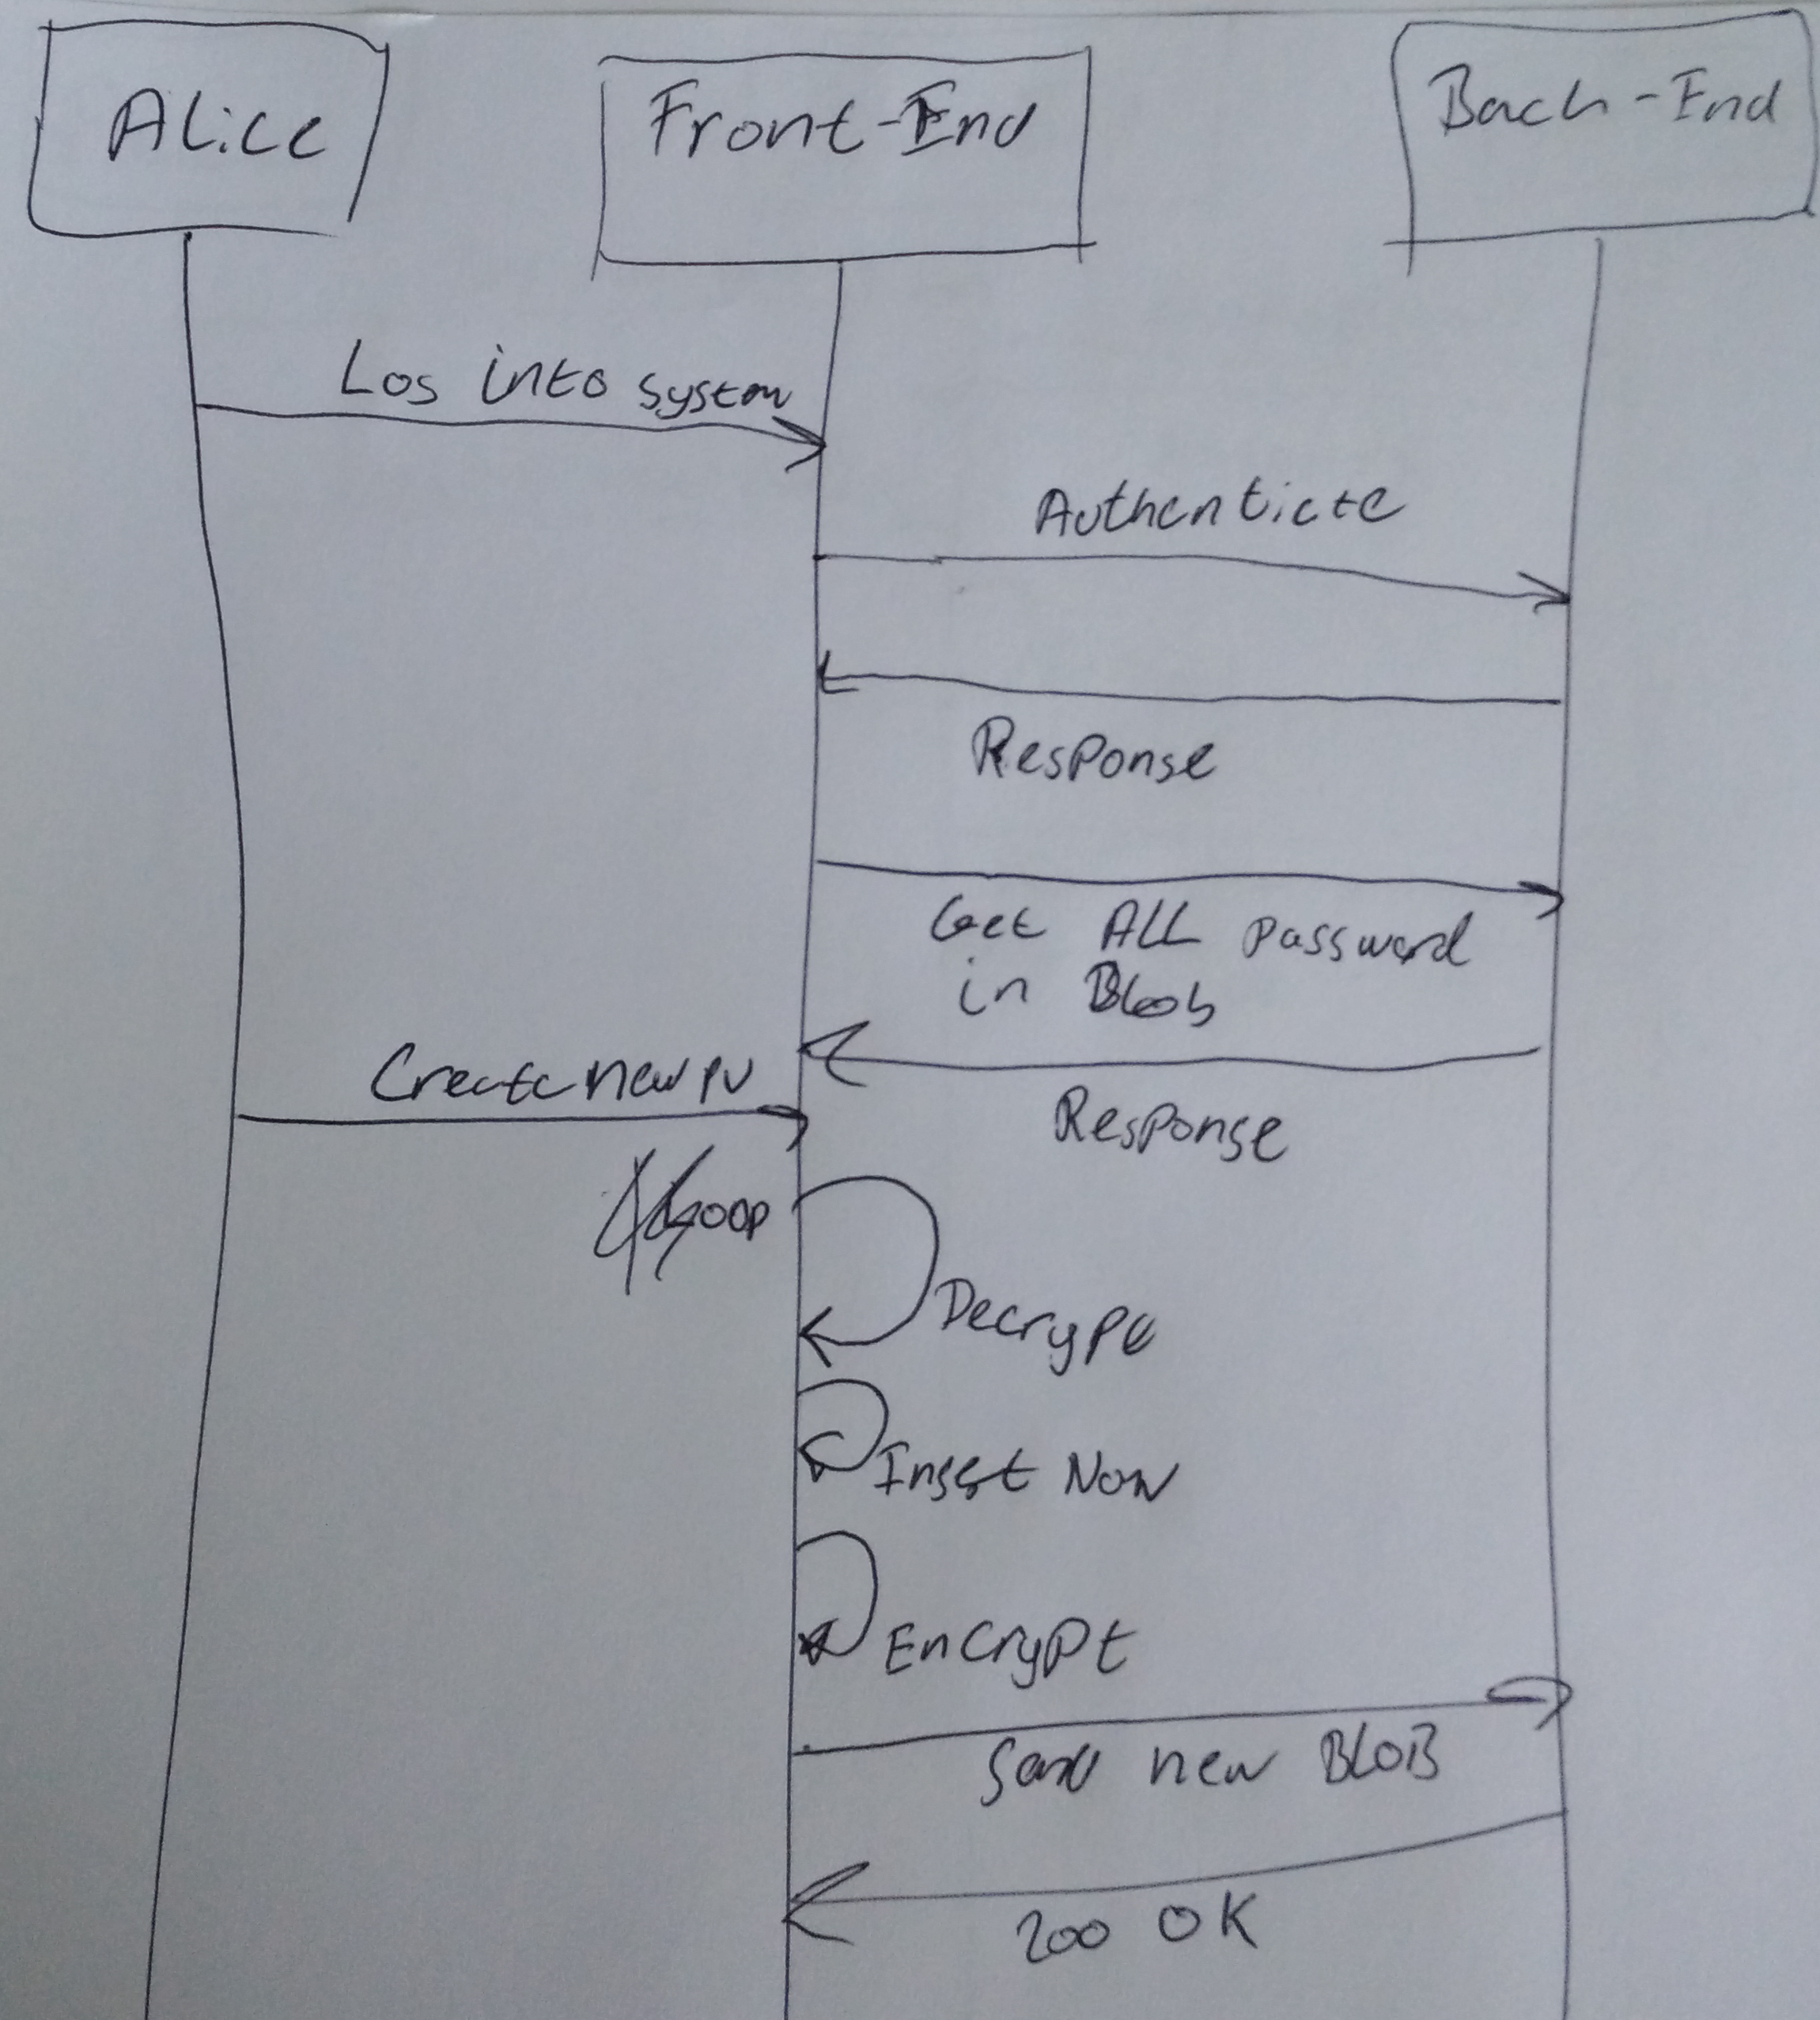
\includegraphics[width=\textwidth]{figures/design/sequence_blob.png}
				\caption{Squence diagram for creating new password using blob encryption.}
				\label{fig:seq_blob}
			\end{figure}

			The advantage to this, is that the blob practically can be encrypted with whichever scheme the user chooses; The back-end merely sends and receives blobs. However, it also has a \emph{major} drawback. This approach, unfortunately, results in a large amounts of overhead: Every time a single entry is accessed, the entire blob needs to be decrypted. Same goes for updating: The entire blob will need to be both decrypted and encrypted again. While this might not be a huge issue with small datasets, it really doesn't scale all that well.


		\subsection{Per Entry Encryption}
			An alternative approach is that encryption could be employed on a per-entry basis. Using this scheme, some of the attributes per entry could then be encrypted. An example of such an entry could be a set consisting of a username, password, and URL. In this specific \emph{example} the password could be the only thing encrypted. 

			Using the same example before, of a password being added or updated, it is clear that encryption-wise, this solution is a lot more lightweight. \emph{Only} the updated / new fields are changed, leaving the remainder of the data unchanged. This sequence of events, is depicted on the sequence diagram on figure \ref{fig:seq_perentry} on page \pageref{fig:seq_perentry}. The drawback to this, is that additional information has the potential of being exposed in the database \emph{(unless the entire entry is encrypted)}.


			\begin{figure}[h!]
				\centering
				\includegraphics[width=\textwidth]{figures/design/na.png}
				\caption{Squence diagram for creating new password using individual.}
				\label{fig:seq_perentry}
			\end{figure}

		\subsection{Sharing is Caring}
			However, deciding the encryption scheme based on the previous sections is not possible. There is one important aspect, not yet considered: As stated in section \ref{sec:requirements} on page \pageref{sec:requirements} being able to share a password is a requirement. As such, it is important that a user, Alice, is able to share a password with another user, Bob -- and \emph{only} Bob.

			For this feature, an encryption scheme is needed which satisfies the following: Alice can share a single password with Bob, without Bob being able to access the remaining passwords. It should happen purely from Alice's part: No interaction with Bob should be necessary before a password is shared.

			\subsubsection{Asymmetric Encryption}
				Using asymmetric encryption, the previous conditions are easily met. Each user has both a private-key and a public-key stored on the server. When Alice wish to share a password with Bob, she requests the server for Bob's public-key. Once she gets this, she then re-encrypts the password with \emph{Bob's} public-key, and sends this to the server. This way, the password is never handles un-encrypted anywhere other than Alice's front-end. Finally, Bob can easily decrypt the password, using his own private-key. This sequence of events, is shown on figure \ref{fig:seq:assymetric} on page \pageref{fig:seq:assymetric}.

				\begin{figure}[h!]
					\centering
					\includegraphics[width=\textwidth]{figures/design/sequence_perEntry.png}
					\caption{Squence diagram for sharing a password, when asymmetric encryption is used.}
					\label{fig:seq:assymetric}
				\end{figure}

				As the astute reader might have already thought of, there is a slight short-coming in what was previously described. The private-key -- the key used for \emph{decrypting} passwords -- is stored on the server. If stored in ``clear text'' \emph{(or raw binary)}, this presents a huge security risk. Not only is the server admin \emph{easily} able to decrypt passwords, but \emph{should} a leak of the database happens, all passwords are instantly compromised.

				As such, it is necessary to introduce some sort of encryption for the private-key. But how can this be achieved without merely shifting the issues previously described? It is necessary to derive the encryption key, from the user's input. Translating a user's input -- for instance a password -- to an encryption key is very common, and is best done using a key derivation function. 

				Algorithms such as bcrypt and PBKDF2 exists for this very purpose \emph{(or slightly similar, at least)}. In layman's terms, it basically hashes the same password over and over again, $n$ times, as to slow the process down ``artificially''. This is done so that trying to bruteforce the key, will be several factors more difficult, due to the extra computations.


				 These algorithms are commonly used for 

				Bcrypt is commonly used for password hashing. Bcrypt




		 One example could be to store all of the users entries in a single file, which is then encrypted using an appropriate algorithm. Another solution could be to store all the entries in database, where certain fields are encrypted and stored as blobs. 

		Both of these solutions are equally valid. However, when examining the second requirement, as previously quoted, password sharing is a requirements. This becomes problematic 




	\section{Authentication}
		\subsection{OAuth1/2}
		\subsection{Basic Authentication}
		\subsection{Tokens}
			\subsubsection{Simple Web Tokens (SWT)}
			\subsubsection{JSON Web Tokens (JWT)}
		
		\subsection{Two-Factor Authentication}

	\section{Securing the API}

	\section{Encryption \& Data Security}
		\subsection{Pseudo Zero Knowledge}


	\section{Storing the Data}
		\section{SQL vs NoSQL}
		\section{SQLite}
	\section{Storage Scheme}

	\section{Naming the Solution}


%\chapter{What Could Go Wrong?}
\chapter{Risks}
	Having described the implementation of the prototype, it is very important to acknowledge any short-comings or dangers in the use of the final solution. As such, in this chapter the greatest risks are discussed.
	

	\section{Weak Authentication and Decryption Passwords}
		One of the most fundamental risks of using this implementation, is if the user chooses a weak password. Granted, this is a weakness that applies to \emph{everything} protected by a weak password.

		If a can be guessed easily, by known publicly available information regarding the user, or can be bruteforced in a reasonable short about of time, they are thought to be weak. Such a password would in the event of an attacker attempting to gain access, result in greater risk of leaking the \emph{actual} passwords.

		Unfortunately, preventive measures for this type of weakness, is fairly useless. Enforcing password policies is how it is often done in critical systems, but more often than not, the resulting password is chosen so it is easy to remember. As such, it is decided that this risk is \emph{completely} up to the user to avoid.

	\section{Identical Encryption and Decryption Passwords}
		In section \ref{sec:design:pseudo-zero-knowledge} on page \pageref{sec:design:pseudo-zero-knowledge} it was discussed why the design of the system requires two passwords. However, at \emph{no} point will the implementation ever actually compare these passwords. As such, it is \emph{completely} possible for the user to have identical authentication and decryption passwords.

		The risk of this, is potentially giving the server owner the ability to decrypt the stored passwords, since the authentication password \emph{is} sent to the back-end, for authentication purposes. However, this all depends on the user's \emph{choice}, and as such is not regarded as a critical risk.
	
	\section{Trusting the Server Owner}
		While the pseudo-zero-knowledge concept introduced in section \ref{sec:design:pseudo-zero-knowledge} on page \pageref{sec:design:pseudo-zero-knowledge} is intended to keep admins from reading all of the users' passwords, there is more to the story.

		The admin, whom is assumed to be the owner of the back-end, \emph{could} change the JavaScript files of the front-end, making them send all the unencrypted data back to him. 

		In \emph{theory} this could be mitigated by publishing a checksum of the bundled JavaScript file, that the front-end executes. This could then be compared, using a separate browser plugin on load, determining whether or not the file had been tampered with.

		However, there is a much more fundamental issue here: Trust. This implementation is meant to be \emph{self-hosted}. The multi-user support is intended to allow multiple users from the same small community or home, e.g. husband and wife, to share the same back-end for storing their private passwords. As such, a certain level of \emph{trust} is assumed. The pseudo-zero-knowledge ensures that the admin can not read the passwords, using information found in the implementation as originally developed. Beyond that, the users will simply have to trust the admin, that he or she will not deliberately alter the files, in order to access their passwords.

	\section{Third Party Libraries}
		As previously stated, the implementation relies on third party libraries, to perform certain functions. For instance, the Forge library is used for handling encryption in the front-end, and the Node-Argon2 library, is used for performing Argon2 password hashing in the back-end. 

		Using these libraries -- or dependencies, as they're called in the Node.js community -- enabled prototypes to be rapidly developed. However, they also introduce a risk: The implementation relies on other people's code. Recently the largest dependency manager for Node.js, npm, experienced a catastrophic event. A very basic package, \verb=left-pad= was removed from npm, due to a legal dispute between the author and a third party\cite{npm_leftpad}. This caused a chain reaction of chaos, as packages that depended on \verb=left-pad= no longer could be installed, and packages depending on those packages couldn't either -- and so forth. This is unfortunately the risk, when working with these kinds of dependencies, but it isn't even the worst.

		When depending on libraries, the developer\emph{(s)} trust that the author\emph{(s)} of the library is forthright about the content of the library. For instance, the Forge library could, for all intents and purposes, simply send every single encryption payload to a remote server. Luckily, since this \emph{is} the world of open source, the source code can be inspected, and security flaws and vulnerabilities possibly found. However, there \emph{might} still be both intentional and unintentional security risks involved with using these libraries. As such, it is the developers duty to assess the quality of \emph{any} dependency used.

	\section{Dumping the Memory}
		Unfortunately, since the implementation is run in a browser, it is not possible to implement features depending on for instance Microsoft's Data Protection Application Programming Interface \emph{(DPAPI)}, like KeePass does. As such, storing the passwords unencrypted is \emph{unfortunately} a security risk.

		There really isn't any way around this risk. For it to be shown to the user, in the browser, it needs to be decrypted. For it to be shown, it needs to be stored. Should an attacker make a dump of the process memory, he or she will \emph{unfortunately} gain access to any passwords decrypted. 

		The same is said about swap partitions and pagefiles. Unfortunately, there is a risk of clear text passwords ending up in these. It is a risk that comes with the choice of implementation. Should it have been chosen to implement native clients instead, this could possibly be circumvented. So this risk, is the price that will have to be paid, for the convenience of a web application.

		Even the encrypted passwords are somewhat at risk. For user experience purposes, the decrypted private key is kept in memory. A mechanism clearing this variable could of course be devised, but that would result in the user having to enter their decryption password \emph{every} time he or she needed to access a password -- which would result in a horrible user experience.


		%So even when removing the decrypted passwords, the encryption key for decrypting \emph{all} passwords, still resides \emph{in memory}. One could of course go about clearing this as well, but that would mean the user would have to enter the decryption password \emph{every} time he or she needed to access a password -- which would result in a horrible user experience.

		%The only redeeming thing to be said about this risk, is the fact that the implementation attempts to remove decrypted passwords again, as soon as possible. When the user changes focus from the password, its variable is overwritten. This is, however, doesn't increase the security all that much. For user experience purposes, the decrypted private key is kept in memory. So even when removing the decrypted passwords, the encryption key for decrypting \emph{all} passwords, still resides \emph{in memory}. One could of course go about clearing this as well, but that would mean the user would have to enter the decryption password \emph{every} time he or she needed to access a password -- which would result in a horrible user experience.

		All in all, this risk is unfortunately unavoidable. It is simply the price paid for the convenience.
	
	\section{Loss of Data in the Database}
		As much as we wish they were, harddrives, flash cards, and USB sticks are fallible. Drive failures \emph{can} -- and eventually \emph{will} -- happen. Unfortunately, not all users will run with a setup supporting parity checks. As such, backing up the database every so often is very much \emph{encouraged}. While this will \emph{not} completely mitigate the threat of data loss, it minimizes the damage done in such an event.

		Backing up the database can easily be done with a cronjob \emph{(or similar)}.

	\section{Leaking the Token}
		In section \ref{sec:design:jwt} on page \pageref{sec:design:jwt} it was decided that the implementation will be using JWT's to handle API authentication. What was \emph{not} discussed, was the security impact this would have.

		When JWTs are used, commonly there is an expiration time set. At the time of this writing, that timer is set to 24 hours, meaning that 24 hours after issuing, the token is no longer valid. As such, after the token is expired the user will need to re-authenticate to access the back-end again.

		However, that also means that should this token fall into the hands of the attacker, he or she will have access to the user's data for 24 hours. This would allow an attacker to change and delete passwords at will, but since password encryption and decryption happens in the browser, he or she will \emph{not} have direct access to the passwords. Avoiding the loss of passwords, can be somewhat mitigated, by backing up the database, as described in the previous section.

		Obtaining these tokens commonly happen through either Cross-Site Request Forgery \emph{(CSRF)} or Cross-Site Scripting \emph{(XSS)}. While there definitely could be security vulnerabilities not found at this point, it is believed that no such exists. Additionally, it is not possible to intercept the token in transit, due to HTTPS being enforced at \emph{all} times.

		As such, the risk of the token being compromised, is relatively low.

		%Another option is to allow for token revocation. This would entail storing the token in the database, allowing the user to revoke tokens at any point in time.


	\section{Forgetting the Password}
		One of the more unfortunate ``issues'' with the implementation, is the lack of account recovery. The authentication password can, \emph{of course}, be reset. But the decryption password can \emph{not} be reset -- for good reasons. As such, if the user forgets his or her decryption password, \emph{nothing} can be done.

		Should this situation arise, it would be unfortunate. But there is nothing that can be done to remedy this risk, that would not lower the overall security of the system. As such, it is deemed a necessary risk.

	\section{Summing Things Up}
		In the previous sections various risks of running the system has been introduced. These range from trusting the owner of the setup, to depending on third party libraries.




		Taken all the risks into consideration, it is still deemed better to deploy the solution as is, rather than trusting remote services with ones password data.

\chapter{Implementation: The Approach}
	Before describing the actual implementation, it is important to describe the process behind it. While this project \emph{is} comparatively small, the main principles of agile development were used. The overall implementation method was iterative: First and foremost, a \emph{very} basic prototype was implemented. This supported nothing more than user authentication, password storage, and password retrieval. The rest of the features were added one by one, until the final prototype was complete.
\input{chapters/implementation/backend.tex}
\chapter{Implementing the System: The Front-End}
	In chapter \ref{chap:impl:backend} the implementation of the back-end was described. In this section, the implementation of the corresponding front-end will be described. It is implemented following the design specifications from chapter \ref{chap:design}.

	\section{Developing for the Browser}
		When developing for the browser, there are three ``possibilities'': JavaScript, Java applets, and Flash. However, from a technological point of view, Flash is horribly outdated. The usage of the Flash plugin has simply declined so much, that it is no longer feasible. Using Java applets are, similarly to Flash, simply outdated. Introducing too many security concerns, issues, and cross-platform issues, this is simply not a good choice.

		This leaves us with JavaScript. This \emph{is} the language that pretty much all interactive web applications are developed today. As such, it is what will be used for this project.


	\section{Using a Framework}
		\begin{itemize}
			\item Angular 1.5
			\item Angular 2.0
			\item ReactJS
			\item Ember
			\item Polymer
		\end{itemize}


	\section{UI-Router}
		\label{sec:impl:ui-router}

	\section{Performing Encryption}

	\section{Generating Passwords}




%\newpage
%\chapter{Todos}
%\todos



\appendix
%\chapter{Stuff and Things}

This appendix is full of stuff ...
%-----------
% Backmatter
%-----------
\backmatter
\chaptermark{Bibliography}
\renewcommand{\sectionmark}[1]{\markright{#1}}
\sectionmark{Bibliography}
\addcontentsline{toc}{chapter}{Bibliography}        %Force addition of Bibliography to TOC
\bibliographystyle{alpha}                           %Use alpha codes for references
\bibliography{references,references/images.bib,references/techpapers.bib,references/design.bib}                           %Bibliography file called

\listoffigures

\end{document}
% % % EOF % % %